\documentclass{nudt}
%%% Bibliography
\usepackage[style=gb7714-2015,hyperref=true,backend=biber,sorting=none,backref=true]{biblatex}
\addbibresource{bibliography.bib}
\begin{document}
% 封面
\begin{titlepage}
	\vspace*{121pt}
	\begin{center}
		\fontsize{30pt}{0} \textbf{\song{优化算法设计与应用}}\\
		\fontsize{30pt}{0} \textbf{\song{实践项目}}\\
		\vspace*{100pt}
		
		\zihao{3}\textbf{\song{名\qquad 称}}:\ \ \underline{\makebox[250pt]{基于改进SA求解VCRP问题}}\\
		\vspace*{72pt}
		
		\zihao{4} \textbf{\song{学员姓名}}:\ \ \underline{\makebox[108pt]{张鑫航}}\ \ \zihao{4}\textbf{\song{专业}}:\ \ \underline{\makebox[108pt]{管理科学与工程}}\\
		\vspace*{5pt}
		\zihao{4} \textbf{\song{学员学号}}:\ \ \underline{\makebox[108pt]{201902001008}}\ \ \zihao{4}\textbf{\song{年级}}:\ \ \underline{\makebox[108pt]{2019级}}\\
		\vspace*{5pt}
		\zihao{4} \textbf{\song{所属学院}}:\ \ \underline{\makebox[270pt]{系统工程学院}} \\
		\vspace*{5pt}
		\zihao{4} \textbf{\song{指导教员}}:\ \ \underline{\makebox[108pt]{杨志伟}}\ \ \zihao{4}\textbf{\song{职称}}:\ \ \underline{\makebox[108pt]{副教授}}\\
		\vspace*{60pt}
		\zihao{-3}\heiti{国防科技大学系统工程学院}
	\end{center}
\end{titlepage} 
\newpage
% 封面
%清除原页眉页脚样式
\fancyhf{} 
\pagenumbering{Roman}
\fancyfoot[CO, CE]{\thepage}
\tableofcontents
%C:页面中间
\fancyhead[CO, CE]{\zihao{-5}优化算法设计与应用实践项目}
\newpage
\pagenumbering{roman}
\fancyfoot[CO, CE]{\thepage}
\begin{abstract}
	车辆路径的优化是供应链优化中的重要环节。本文设计了一种
	改进的模拟退火算法用于求解有客户需求、车辆最大载重量
	的车辆路径问题。运用交换算子和逆转算子
	2种邻域生成算子,采用基本的指数降温方式控制降温过程。
	主要改进在于:
	\begin{enumerate}
		\item 编码方案采用客户编号的顺序编码,
		并设计专门的解码方法\cite{wuyanqun}能够把2种约束全都纳入考虑。
		\item 在优化算法的多水平参数优化试验中,将参数和对应解的关系看作
		高斯过程。
		\item 设置了经验参数优化、贝叶斯参数优化两种参数优化试验,获取了
	对于结果改进较为明显的参数,(其中经验参数优化试验采用并行计算的方式提升了试验效率)。
		\item 添加了每辆车行驶路径的TSP问题的优化。
		\item 设置最大迭代次数提升了算法运行效率。
	\end{enumerate}

	由参数优化试验得到2种共21组较优的参数,依据这些参数求出所有
	问题的解,最终筛选出2组结果相差不大参数:经验参数$T_0=500,\ \alpha=0.85,\ num_{Tk}=7$和
	贝叶斯优化参数$T_0=47.63,\ \alpha=0.9173,\ num_{Tk}=5.801$。
	
	选择贝叶斯优化参数
	$T_0=47.63,\ \alpha=0.9173,\ num_{Tk}=5.801$的结果得到文件中
	所有VRP问题的路径和最短距离。一些问题的解已经接近文件所给出
	的最优解。相距最少的A-n33-k5、A-n33-k6、A-n34-k5、A-n44-k6、A-n45-k7
	基本已经达到文件所给最优解见下表。其他问题的误差也控制在$3\%$以内。
	所有问题的路径和最优解见\ref{appendix:bayesVRP}。
	% Table generated by Excel2LaTeX from sheet '误差'
	\begin{table}[htbp]
	\centering
	  \begin{tabular}{ccccccc}
	  \toprule
	  VRP问题 & SA最优解 & 文件最优解 &     & VRP问题 & SA最优解 & 文件最优解 \\
	  \midrule
	  A-n33-k5 & 662 & 661 &     & A-n44-k7 & 938 & 937 \\
	  A-n33-k6 & 744 & 742 &     & A-n45-k7 & 1146 & 1146 \\
	  A-n34-k5 & 780 & 778 &     &     &     &  \\
	  \bottomrule
	  \end{tabular}%
  \end{table}%
\keywords{CVRP\quad  模拟退火算法\quad   并行计算\quad  贝叶斯优化\quad	分支定界法}

小组分工如下:
\begin{table}[H]
	\centering
	\begin{tabular}{@{}cccc@{}}
	\toprule
	姓名  & 学号           & \multicolumn{2}{c}{分工} \\ \midrule
	\multirow{2}{*}{张鑫航} & \multirow{2}{*}{201902001008} & \multirow{2}{*}{组长} & \multirow{2}{*}{\begin{tabular}[c]{@{}c@{}}建模、基本SA的编写、贝叶斯参数优化试验、\\ 画图、写文章、SA的改进\end{tabular}} \\
		&              &       &                \\
	胡兢  & 201902010006 & 组员    & 建模、经验参数优化试验、基本SA    \\
	\bottomrule
	\end{tabular}
	\end{table}
\end{abstract}
\pagenumbering{arabic}
\fancyfoot[CO, CE]{\thepage}

\section{问题分析}
车辆路径问题(Vehicle Routing Problem,VRP),如\cref{fig:VRP_show},指存在一定数量的客户,
各自有不同数量的货物需求,配送中心向客户提供货物,由一个车队负责运送货物,要求在满足一定的约束
下,设计适当的配送路径,目标是使所有客户的需求都能得到满足,同时达到诸如路程最短、成本最小、耗费时
间最少等目的。
\begin{figure}[H]
	\centering
	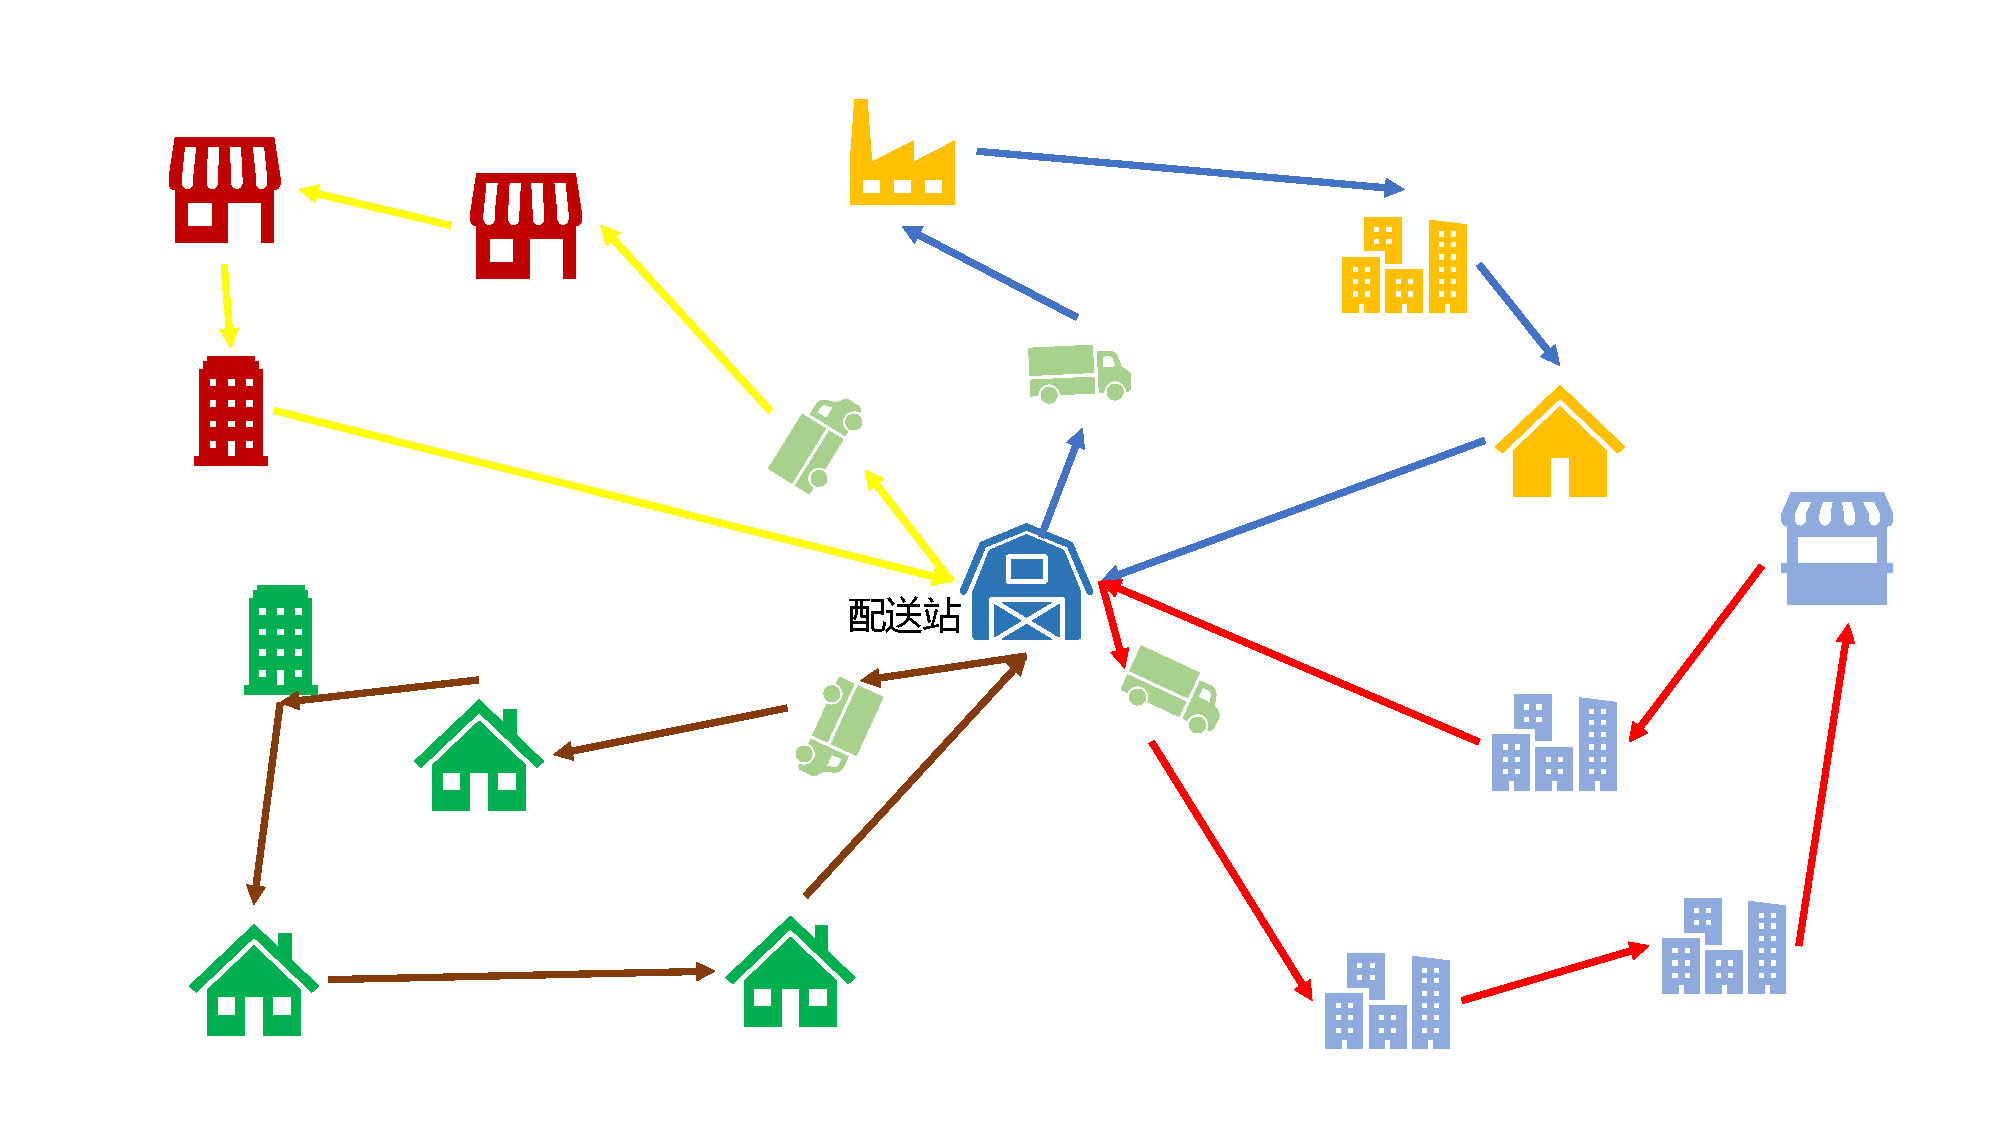
\includegraphics[width = 0.80\textwidth]{image/示意图.pdf}
	\caption{VRP问题示意图}
	\label{fig:VRP_show}
\end{figure}
由此定义不难看出,旅行商问题(Traveling Saleman Problem,TSP)是VRP的特例。
由于Gaery已证明TSP问题是NP难题\cite{1997Heuristic},因此,VRP也属于NP难题\cite{vrpNP}。
\subsection{具有容量限制的路径优化问题(CVPR)}
设有一配送中心(depot),配有多辆货车,有多位客户(customer),
每位客户有其需求量。车辆从配送中心出发对客户进行配送服务最后返回
配送中心,要求所有客户都被配送,每位客户一次配送完成,
且不能违反车辆容量的限制,目的是所有车辆路线的总距离最小。

将上述要求归纳可以得到:
\begin{enumerate}
	\item 每个车辆都要访问配送中心
	\item 每个客户需要被一个车辆服务
	\item 每个路径上,客户的总需求不要超过车辆的容量$Q$ 
	\item CVPR的目标是最小化总路径成本
\end{enumerate}

\section{问题建模}
\subsection{符号说明}
为了方便说明和求解,我们有如下符号说明
\begin{table}[htbp]
	\centering
	\caption{符号说明}
	  \begin{tabular}{cc}
	  \toprule
	  符号  & 意义 \\
	  \midrule
	  $\Lambda$ & 客户顺序的一个排列 \\
	  $\Lambda_{i}\, ,(i=0,1,2,\cdots ,M)$ & $\Lambda$的不相容子列加上depot节点,构成一个解 \\
	  $\Lambda_{i}^{'}$ & $\Lambda$的不相容子列 \\
	  $d_{\lambda_{i,j},\lambda_{i,j+1}}$ & 第$i$辆车经过边$j\rightarrow j+1$的距离 \\
	  $demand_{\lambda_{ij}}$ & 顾客$\lambda_{ij}$的需求量 \\
	  $W\_max$ & 货车最大载货量 \\
	  $M$ & 需要的车的数量 \\
	  \bottomrule
	  \end{tabular}%
	\label{tab:notations}%
  \end{table}%
  
\subsection{问题模型}
\begin{definition}\label{def:xulie}
	$\Lambda = \langle \lambda_1,\lambda_2,\cdots, \lambda_N \rangle $为客户顺序的一个排列。\cite{wuyanqun}
\end{definition}
将$\Lambda$拆开分为$M$个互不相容的子列,并且加上节点$0$,可构造一组问题的解。
\begin{equation}\label{eq:lambda}
	\Lambda_i = \langle 0, \lambda_{i1},\lambda_{i2},\cdots, \lambda_{im_i},0 \rangle
	\, ,(i=0,1,2,\cdots ,M)
\end{equation}
其中$M$代表需要$M$辆车,记
\[
\Lambda_i^{'}=\langle \lambda_{i1},\lambda_{i2},\cdots, \lambda_{im_i} \rangle
\]
\cref{eq:lambda}去除掉首尾的$0$满足
\begin{equation}\label{eq:singlecar}
	\Lambda_i^{'} \bigcap \Lambda_j^{'} = \varnothing
\end{equation}
\cref{eq:singlecar}表示不同车辆经过的节点没有交集。

那么$M$辆车走过的子列的全程距离$z$有
\[
	z = \sum\limits_{i=1}^{M}\sum\limits_{j = 0}^{m_{i}}d_{\lambda_{i,j},\lambda_{i,j+1}}
\]
其中,$d_{\lambda_{i,j},\lambda_{i,j+1}}$代表节点第$i$辆车从节点$\lambda_{i,j}$到$\lambda_{i,j+1}$的距离。

对于某一条路径$\Lambda_i$要满足客户总需求不超过$W\_max$,有
\[
	\sum\limits_{j = 0}^{m_{i}}demand_{\lambda_{ij}}\leqslant W\_max
\]
其中,$demand_{\lambda_{ij}}$代表节点$j$的需求量。
那么有模型如下:
\[
	\min z = \sum\limits_{i=1}^{M}\sum\limits_{j = 0}^{m_{i}}d_{\lambda_{i,j},\lambda_{i,j+1}}
\]
\[s.t.\left\{
	\begin{array}{l}
		\Lambda_i^{'} \bigcap \Lambda_j^{'} = \varnothing \\
		\sum\limits_{j = 0}^{m_{i}}demand_{\lambda_{ij}}\leqslant W\_max
	\end{array}
	\right.
\]

\section{经典的模拟退火算法}
物理退火流程如\cref{fig:physics_a},在升温-等温-降温过程中,粒子共做三种运动:
\begin{description}
	\item[升温]:例子拜托非均匀运动状态 
	\item[等温]:特定温度下粒子趋向平衡态的运动
	\item[降温]:粒子去向稳定态的运动  
\end{description}
模拟退火算法就是将目标函数作为能量函数,当能量函数达到最小,目标函数也最小。
\begin{figure}[H]
	\centering
	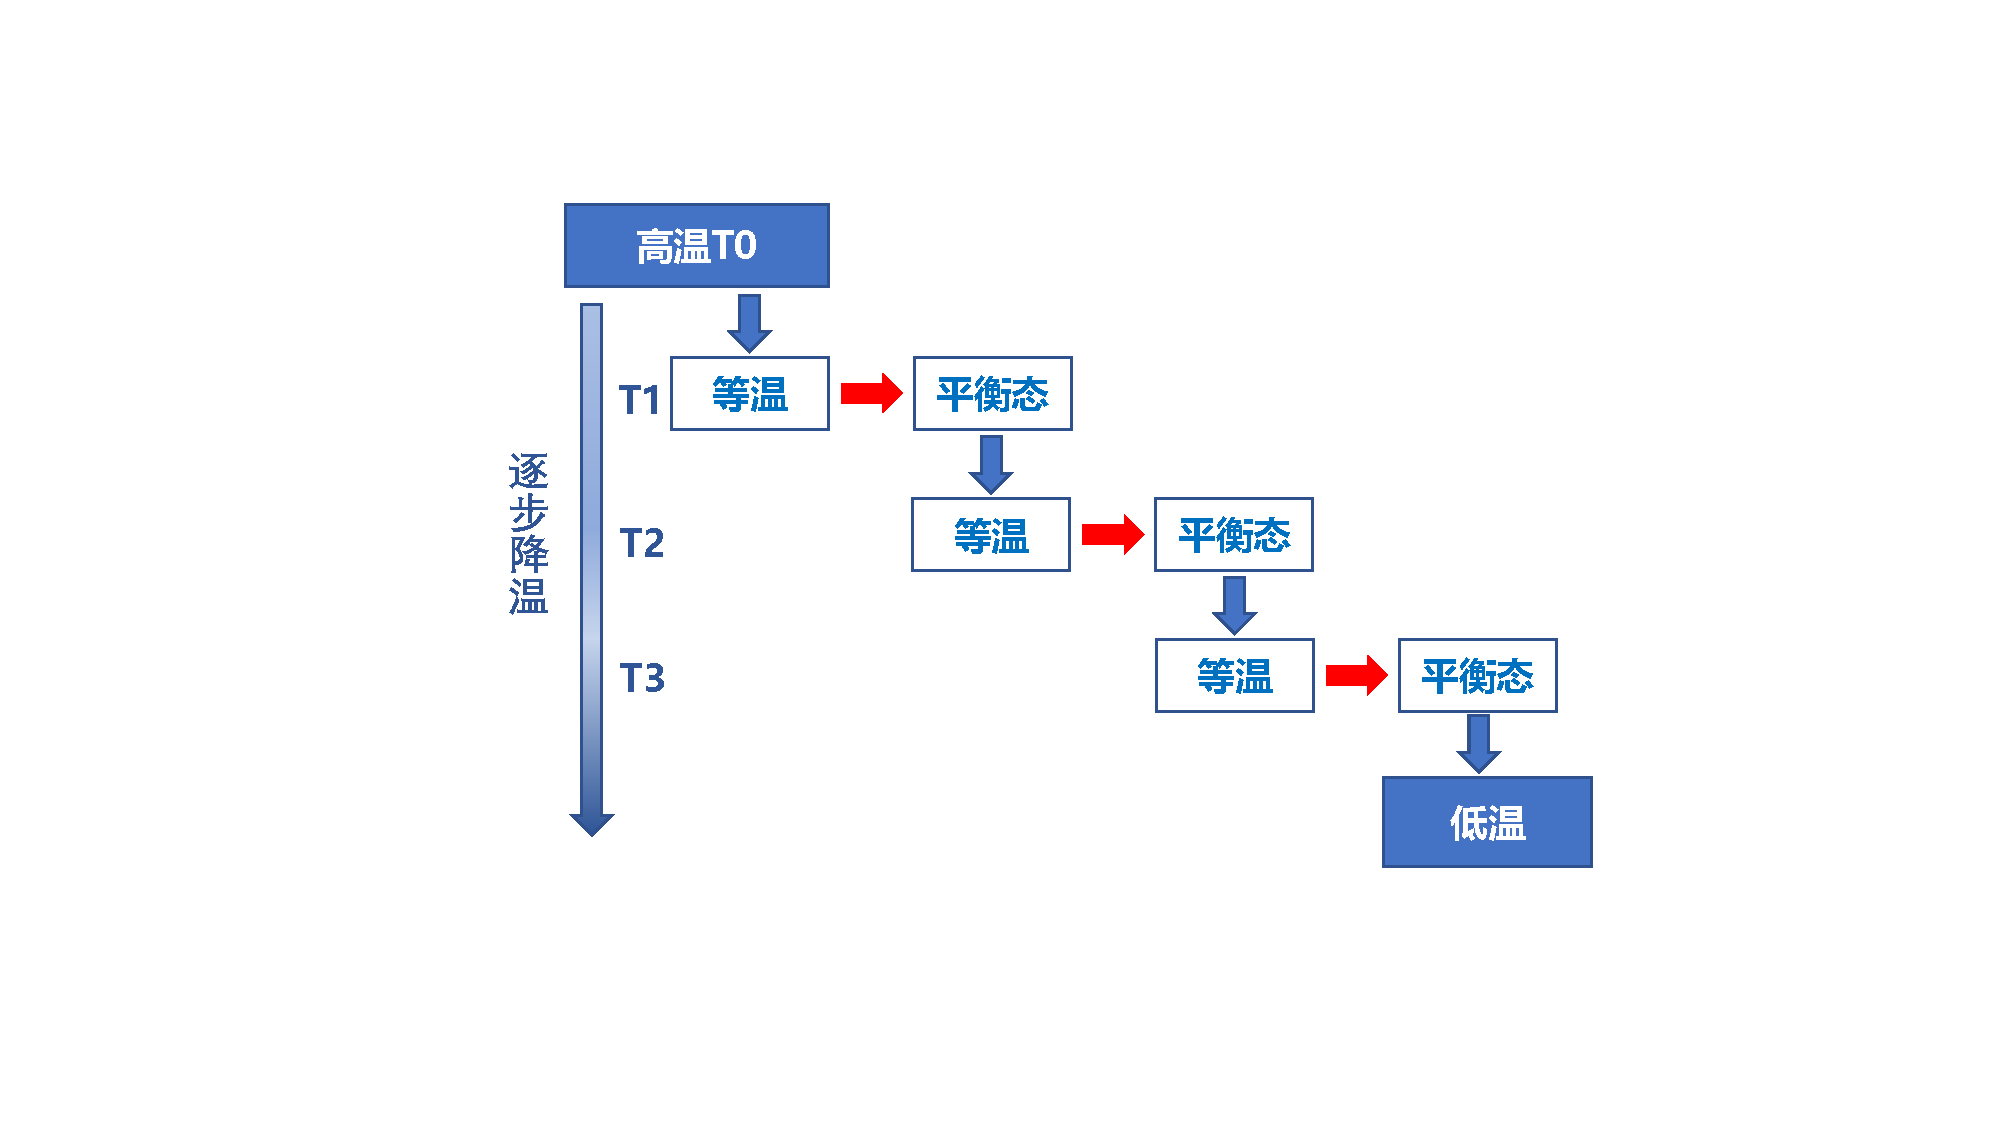
\includegraphics[width=0.75\textwidth]{image/A.pdf}
	\caption{物理退火过程}
	\label{fig:physics_a}
\end{figure}
\subsection{算法流程和实现}
物理退火各个步骤对应到算法如\cref{fig:a2SA},等温到平衡态相当于
局部搜索,可以按照Metropolis准则接受劣解,最终降温
循环得到粒子能量最低的状态。
\begin{figure}[H]
	\centering
	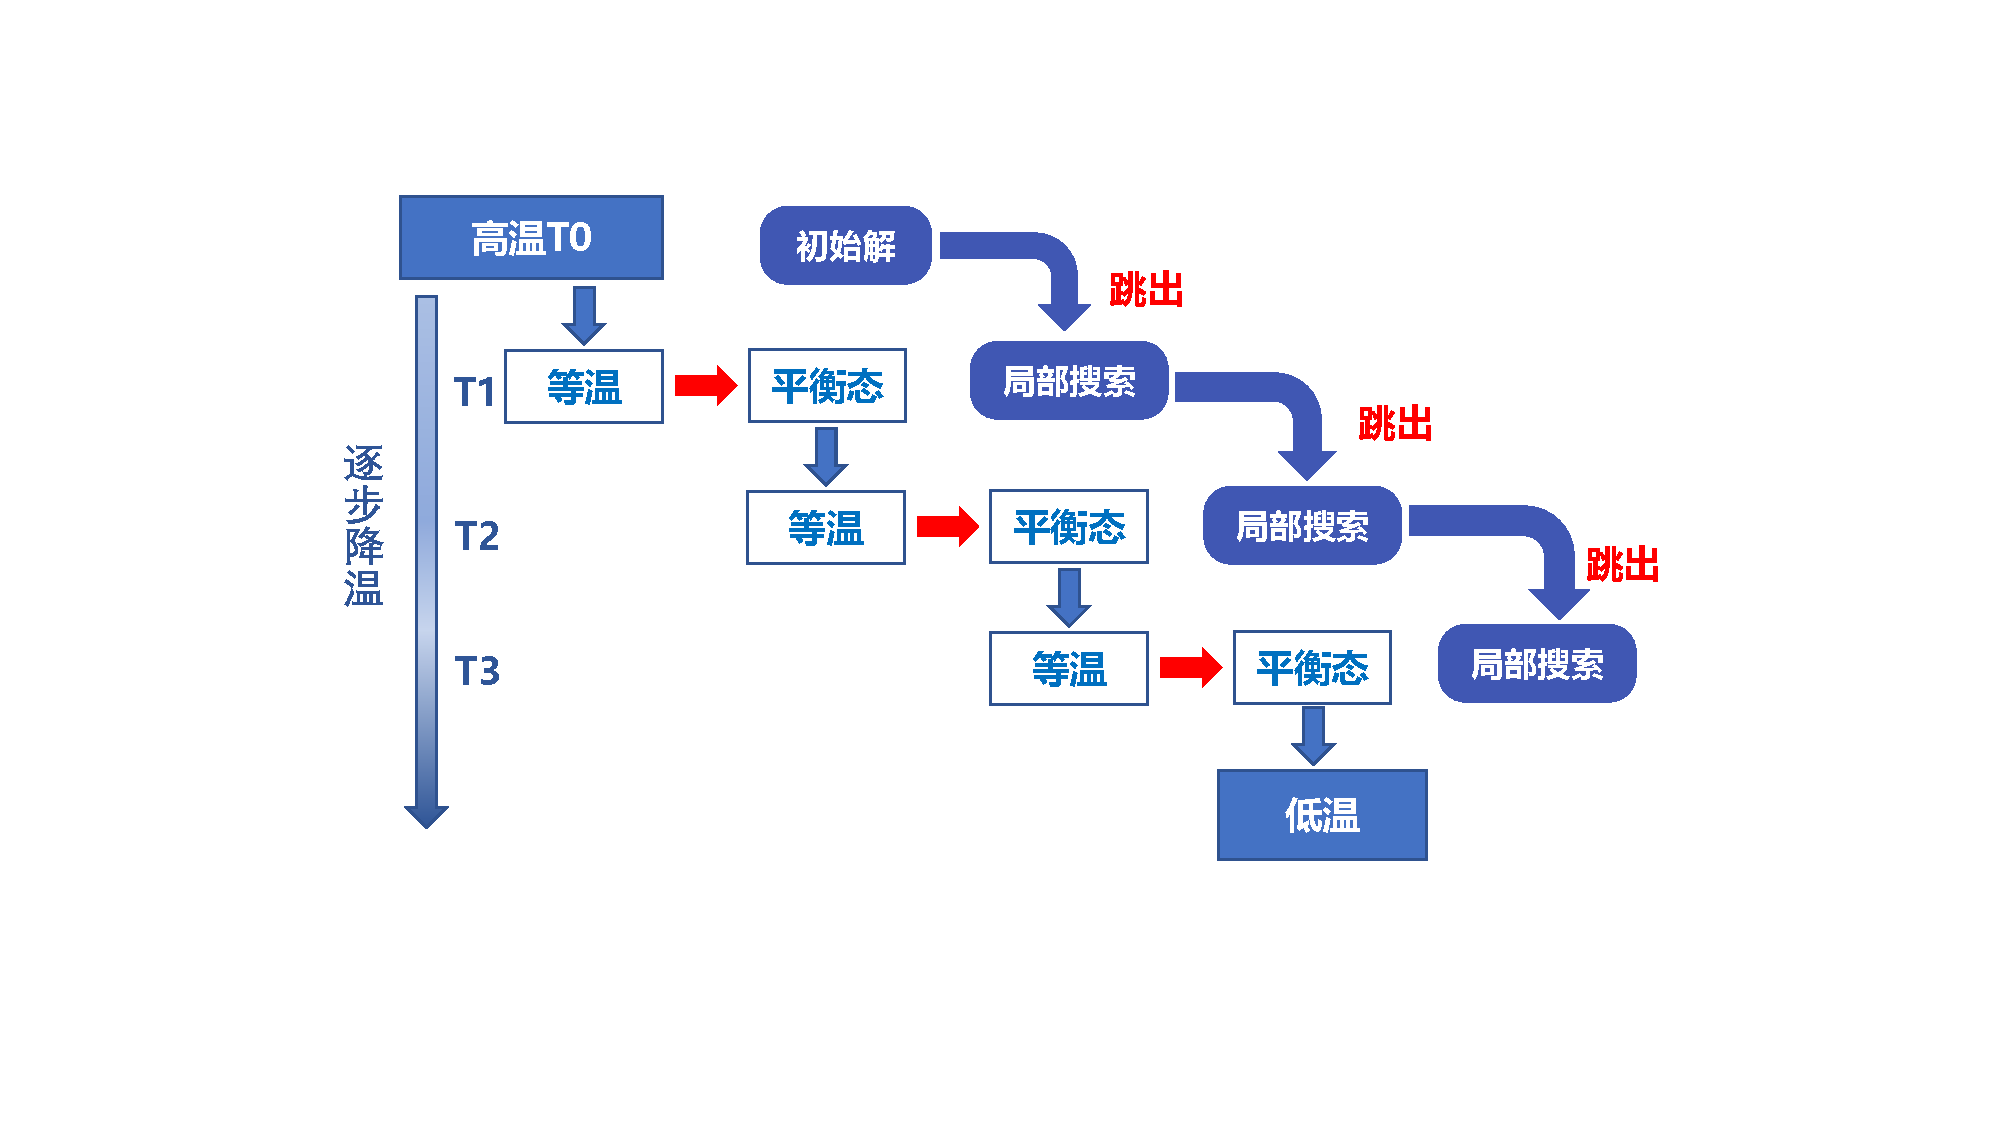
\includegraphics[width=0.80\textwidth]{image/a2sa.pdf}
	\caption{算法对应关系}
	\label{fig:a2SA}
\end{figure}
\subsubsection{实现流程}
模拟退火算法的流程如\cref{fig:SA}:按照Metropolis抽样准则如\cref{eq:Metropolis}
\begin{equation}\label{eq:Metropolis}
	p\left( Tk,s,s^{'} \right) = \left\{ \begin{array}{lr}
		1&		if\,\,f\left( s^{'} \right) \le f\left( s \right)\\
		\exp{\dfrac{f\left( s \right) -f\left( s^{'} \right)}{Tk}}&		others\\
	\end{array} \right. 
\end{equation}
\begin{figure}[H]
	\centering
	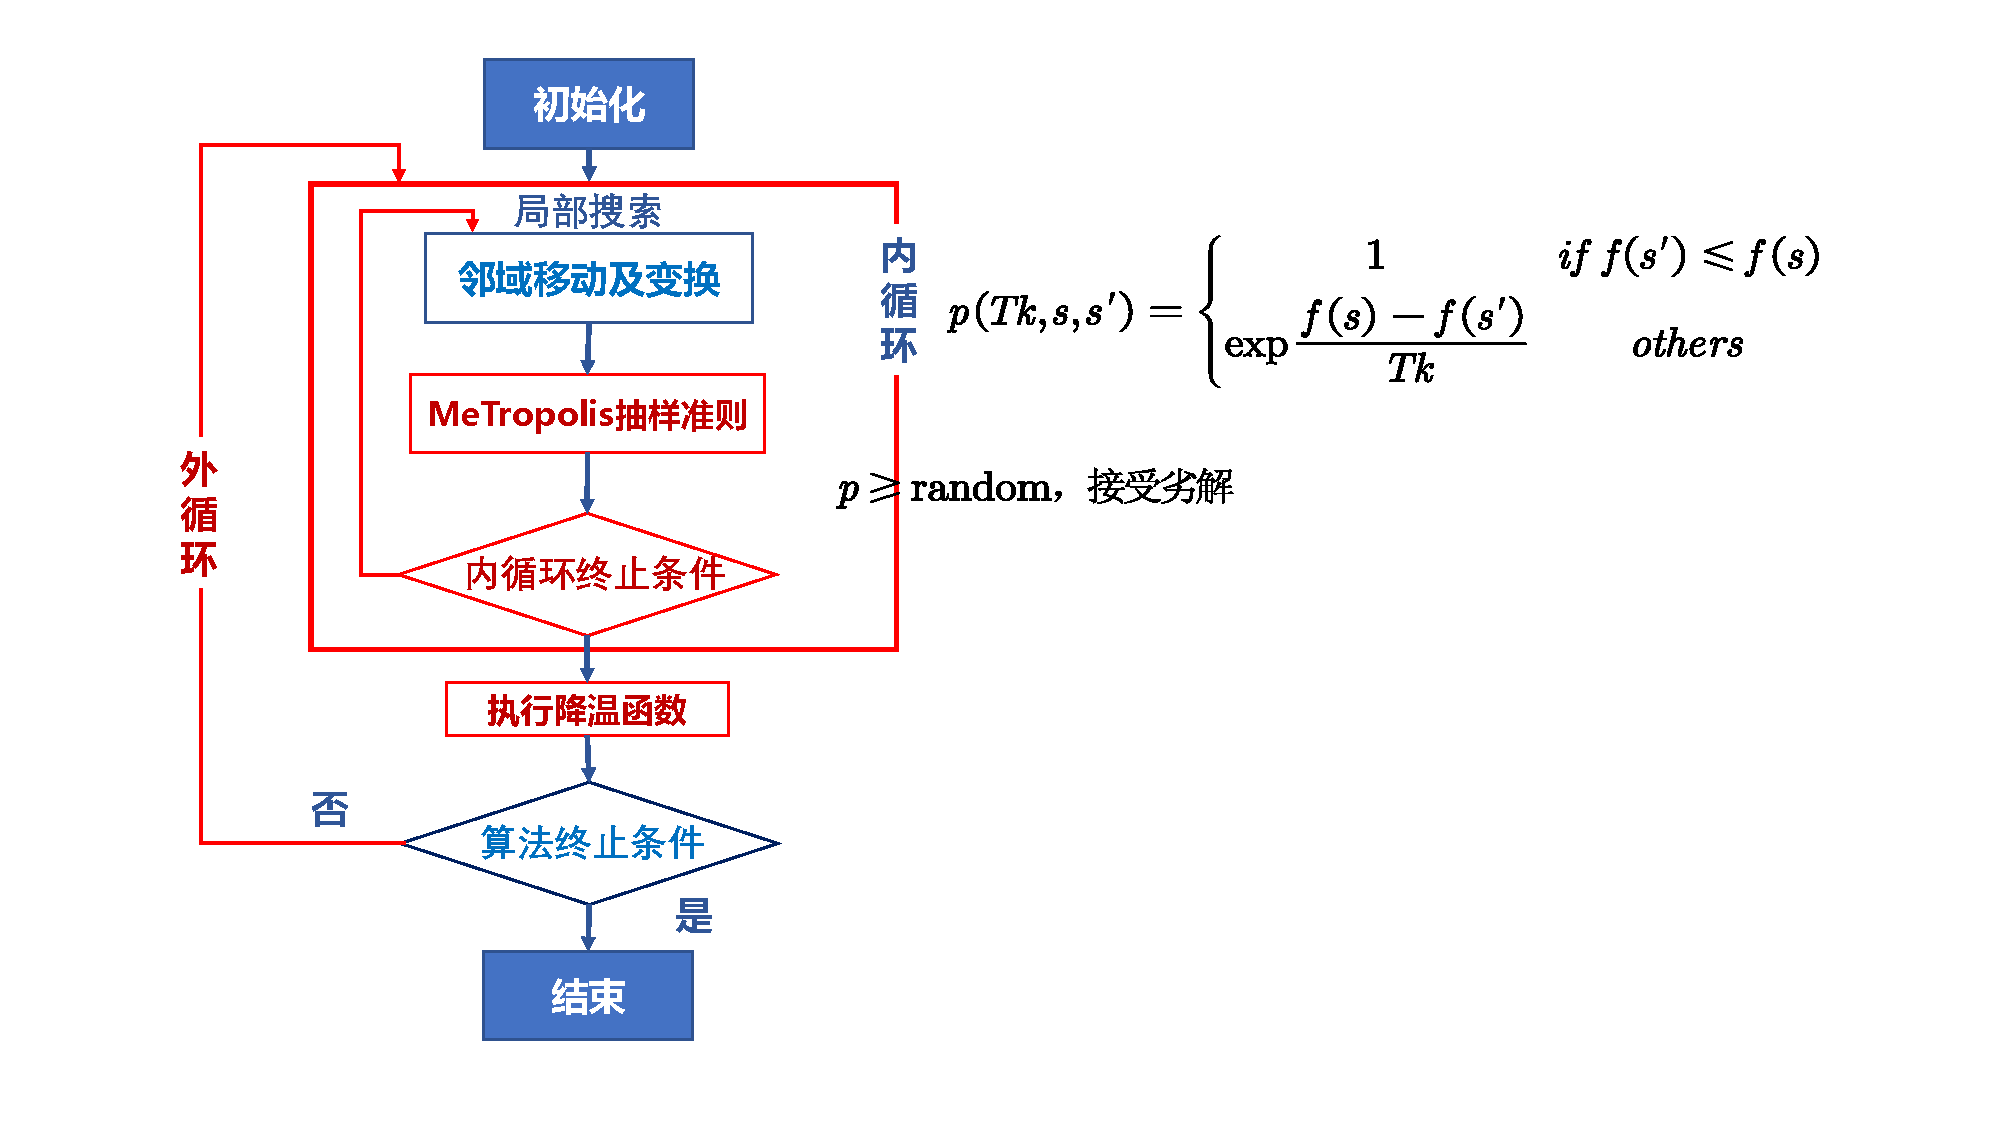
\includegraphics[width=\textwidth]{image/tenser.pdf}
	\caption{模拟退火算法流程图}
	\label{fig:SA}
\end{figure}
\subsubsection{实现的伪代码}
\begin{algorithm}[H]
	\caption{基本模拟退火算法}  
	\label{alg:Basic SA}
	\begin{algorithmic}[1] %每行显示行号  
		\Require $node\_id$节点id数组,$coord$节点坐标数组,$demand$需求数组,$vehicle\_cap$货车载量 
		\Ensure $num\_cars$车辆数目,$routes$车辆路径数组,$obj$最终距离  
		\Procedure{SA}{$node\_id, coord, demand, vehicle\_cap$}   
		\State $sol \gets Sol()$
			\While{$Tk\geqslant T_{end}$ \textbf{and} $iter\leqslant max\_iter$}  
				\For{$i = 0 \to num\_T\_k$} 
					\State $new\_sol \gets Sol()$ 
					\State $new\_sol.nodes\_seq \gets Do\_Action(sol.nodes\_seq, action\_list)$ 
					\State $new\_sol.obj, new\_sol.routes \gets Cal\_Obj(new\_sol.nodes\_seq)$
					\State $ \Delta f \gets new\_sol.obj - sol.obj $
					\If{$\Delta f < 0\ \textbf{or}\ e^{-\frac{\Delta f}{Tk}} > random$} 
						\State $sol \gets new\_sol$
					\EndIf
					\If{$sol.obj < model.best\_sol.obj$} 
						\State $sol \gets new\_sol$
						\State $sa.best\_sol \gets sol$
					\EndIf
				\EndFor
			\If {$\alpha<1$}
				$Tk\gets Tk\times \alpha$
			\EndIf
			\If {$\alpha>1$}
			$Tk\gets Tk- \alpha$
			\EndIf
			\EndWhile   
		\EndProcedure  
	\end{algorithmic}  
\end{algorithm} 
其中产生的邻域的算子,参考文献\cite{wuling}我们选取交换算子和逆转算子如\cref{fig:suanzi}。

采用两种降温方式,线性降温和指数降温如\cref{eq:temp},以方便我们之后进行试验选取最优降温策略和初始温度。
\begin{equation}\label{eq:temp}
	\left\{
		\begin{array}{lr}
			T_{k+1}=\alpha T_{k}, &  \alpha<1\\
			T_{k+1}=T_{k}-\alpha, &  \alpha>1
		\end{array}
		\right.
\end{equation}
\begin{figure}[H]
	\centering
	\begin{subfigure}{\linewidth}
		\centering
		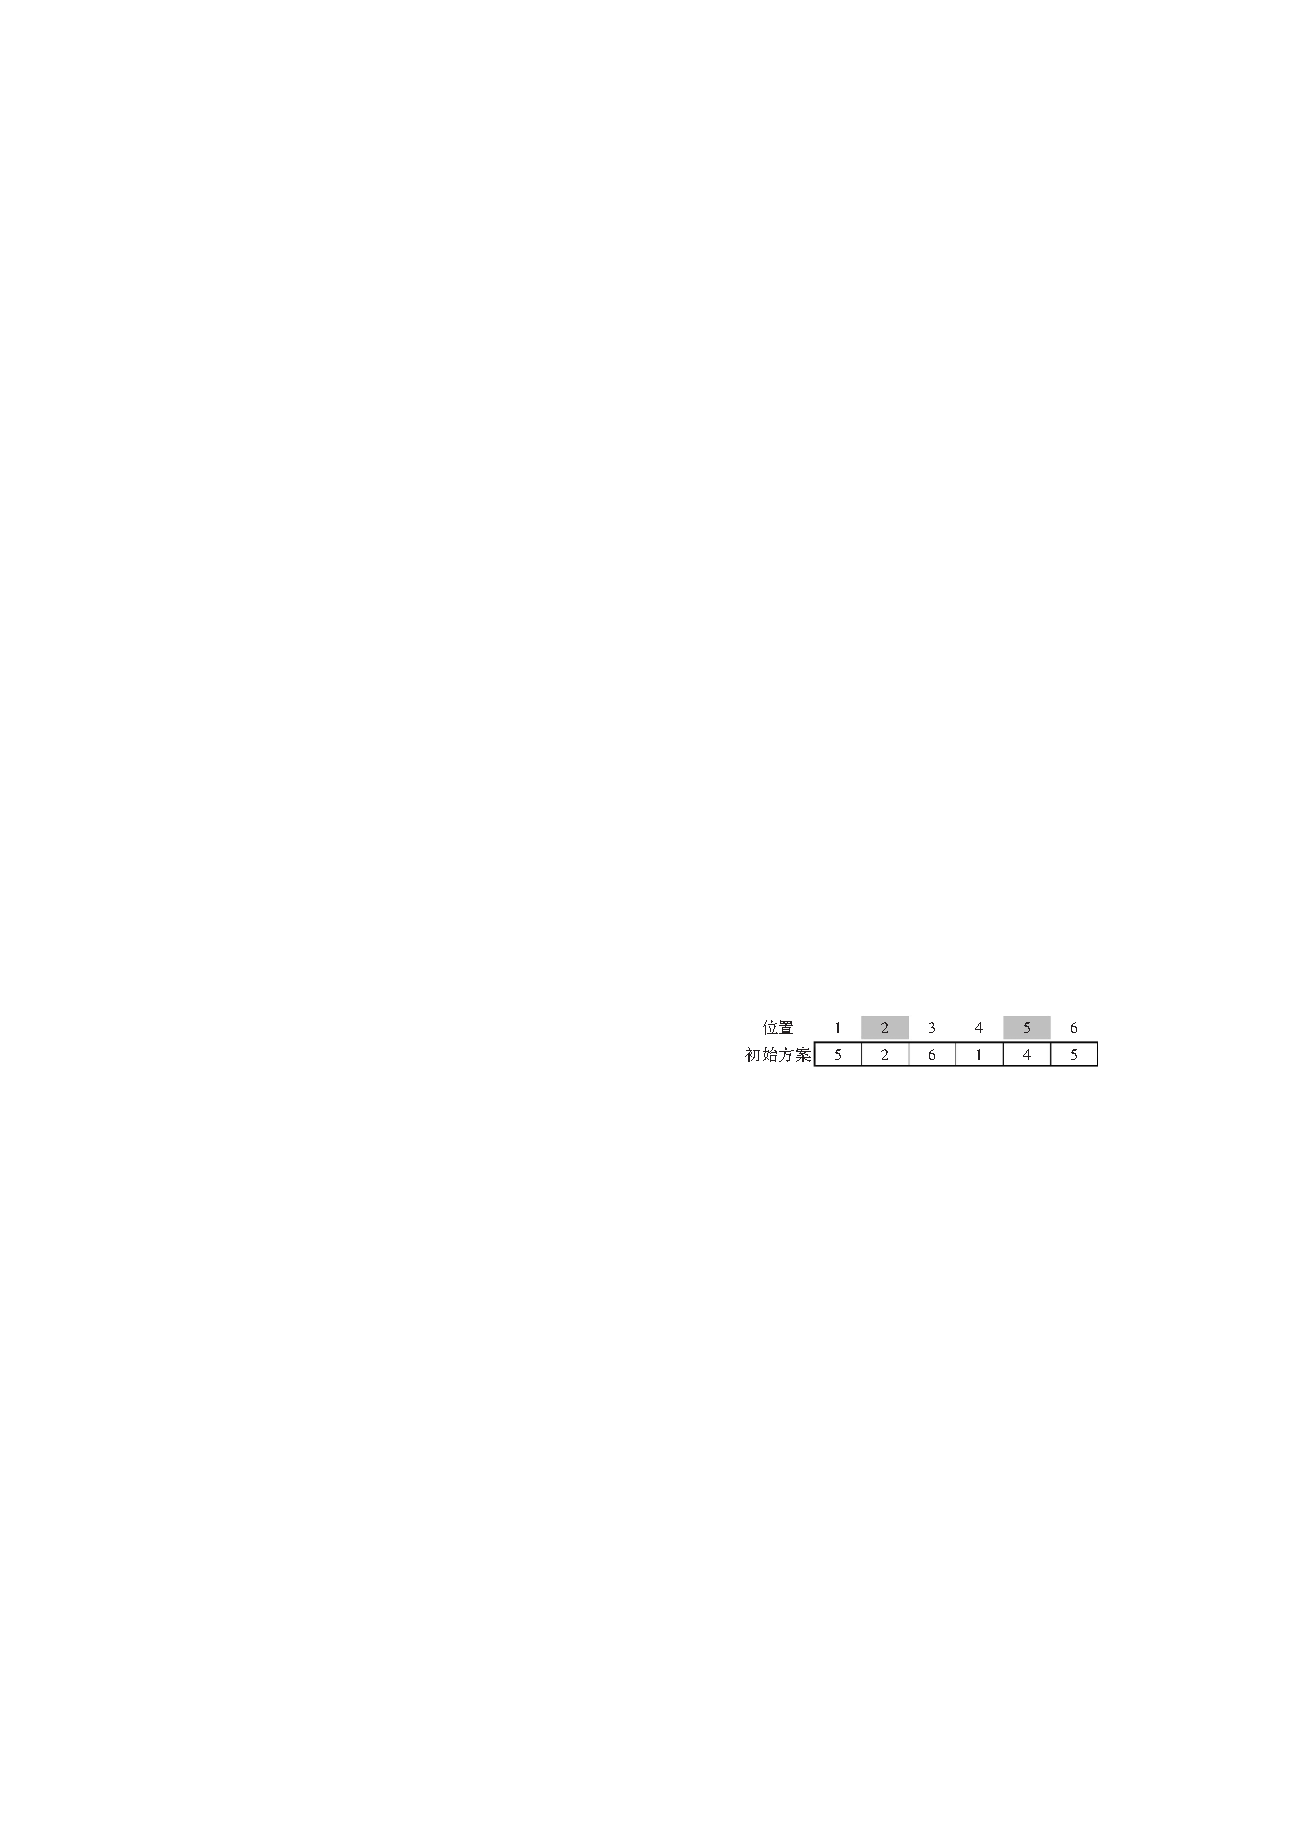
\includegraphics[width=0.75\textwidth]{image/算子.pdf}
		\caption{例子}
		\label{fig:example}%文中引用该图片代号
	\end{subfigure}
	\centering
	\begin{subfigure}{0.325\linewidth}
		\centering
		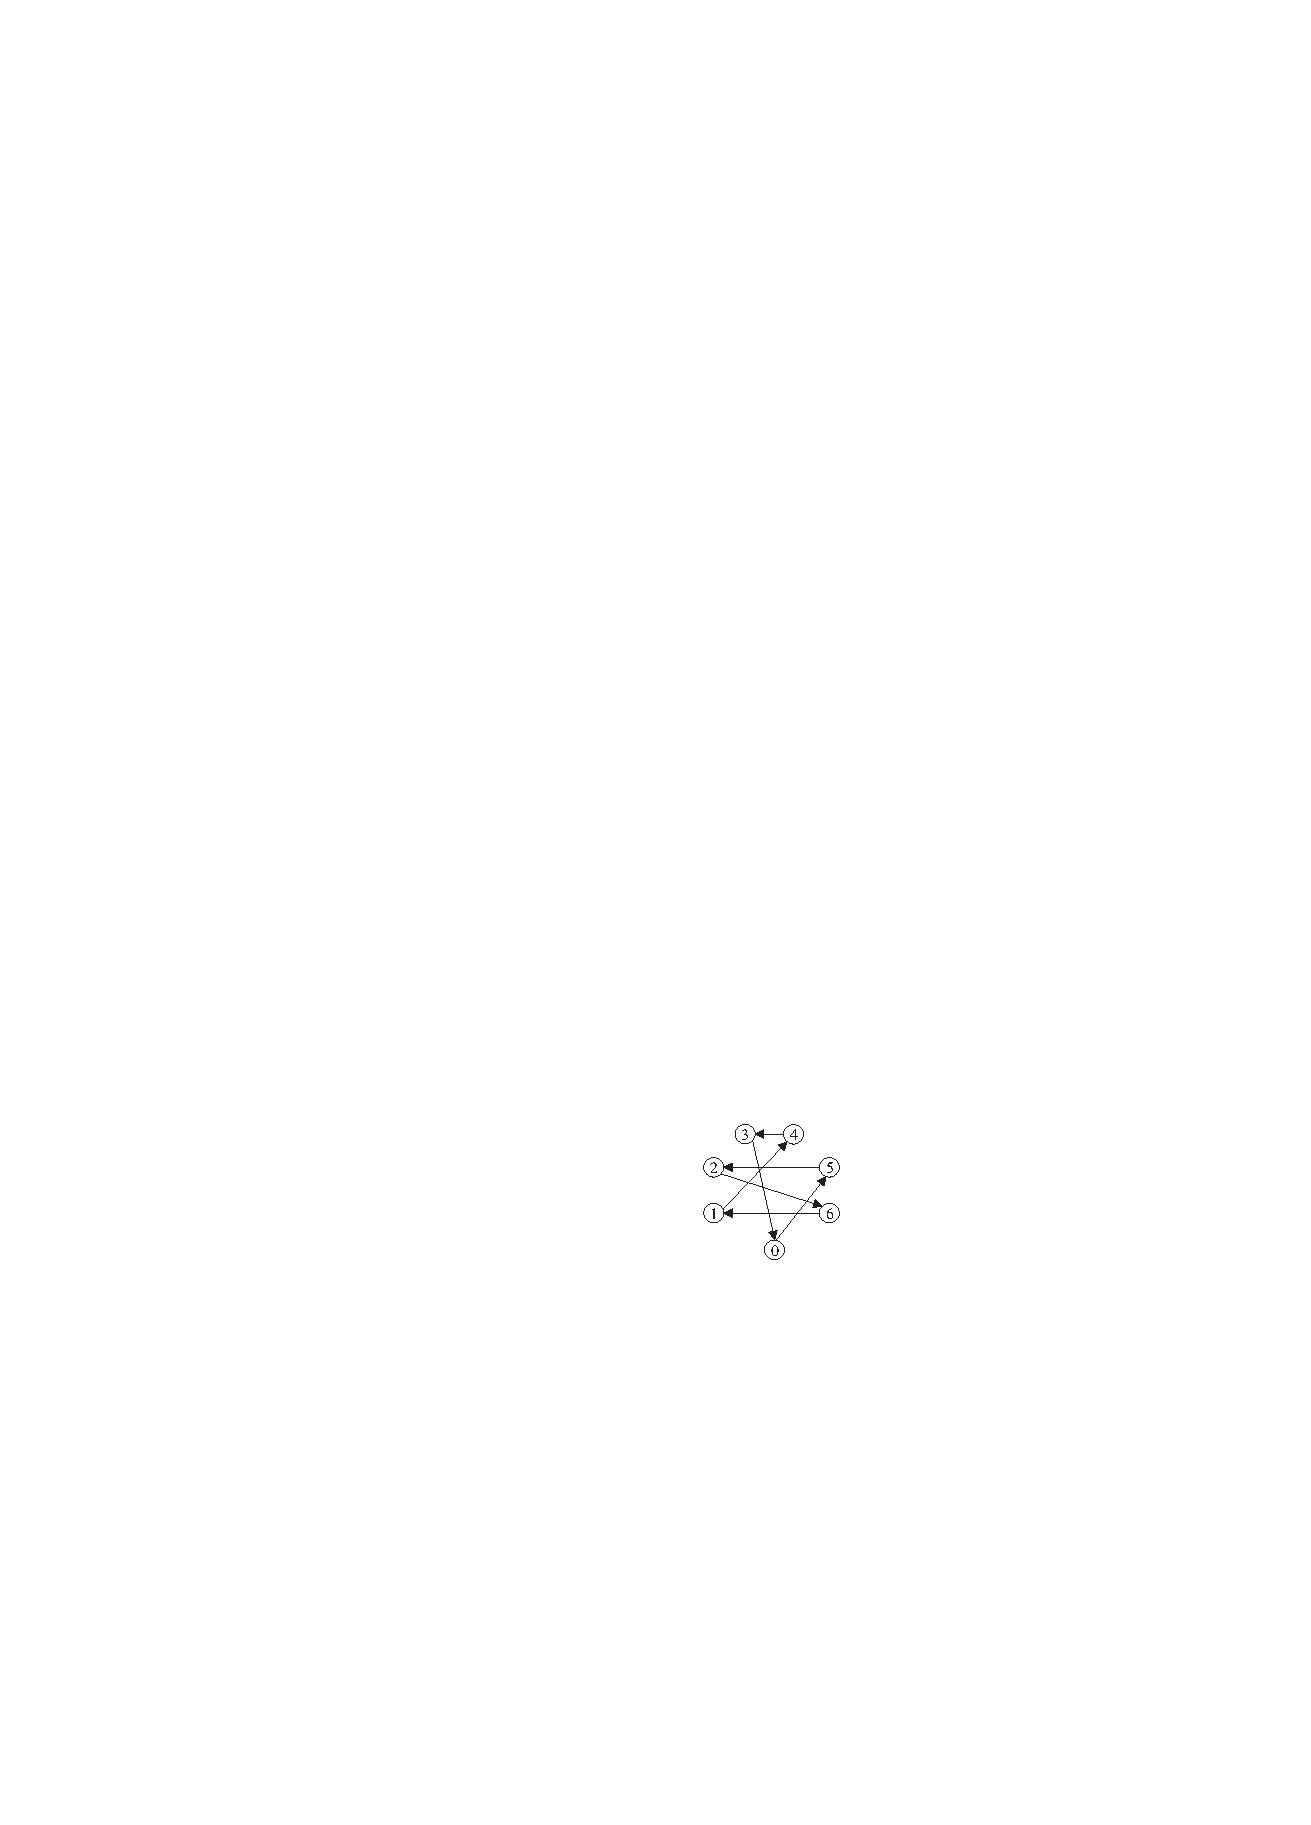
\includegraphics[height=0.75\linewidth]{image/原始.pdf}
		\caption{原始}
		\label{fig:before}%文中引用该图片代号
	\end{subfigure}
	\centering
	\begin{subfigure}{0.325\linewidth}
		\centering
		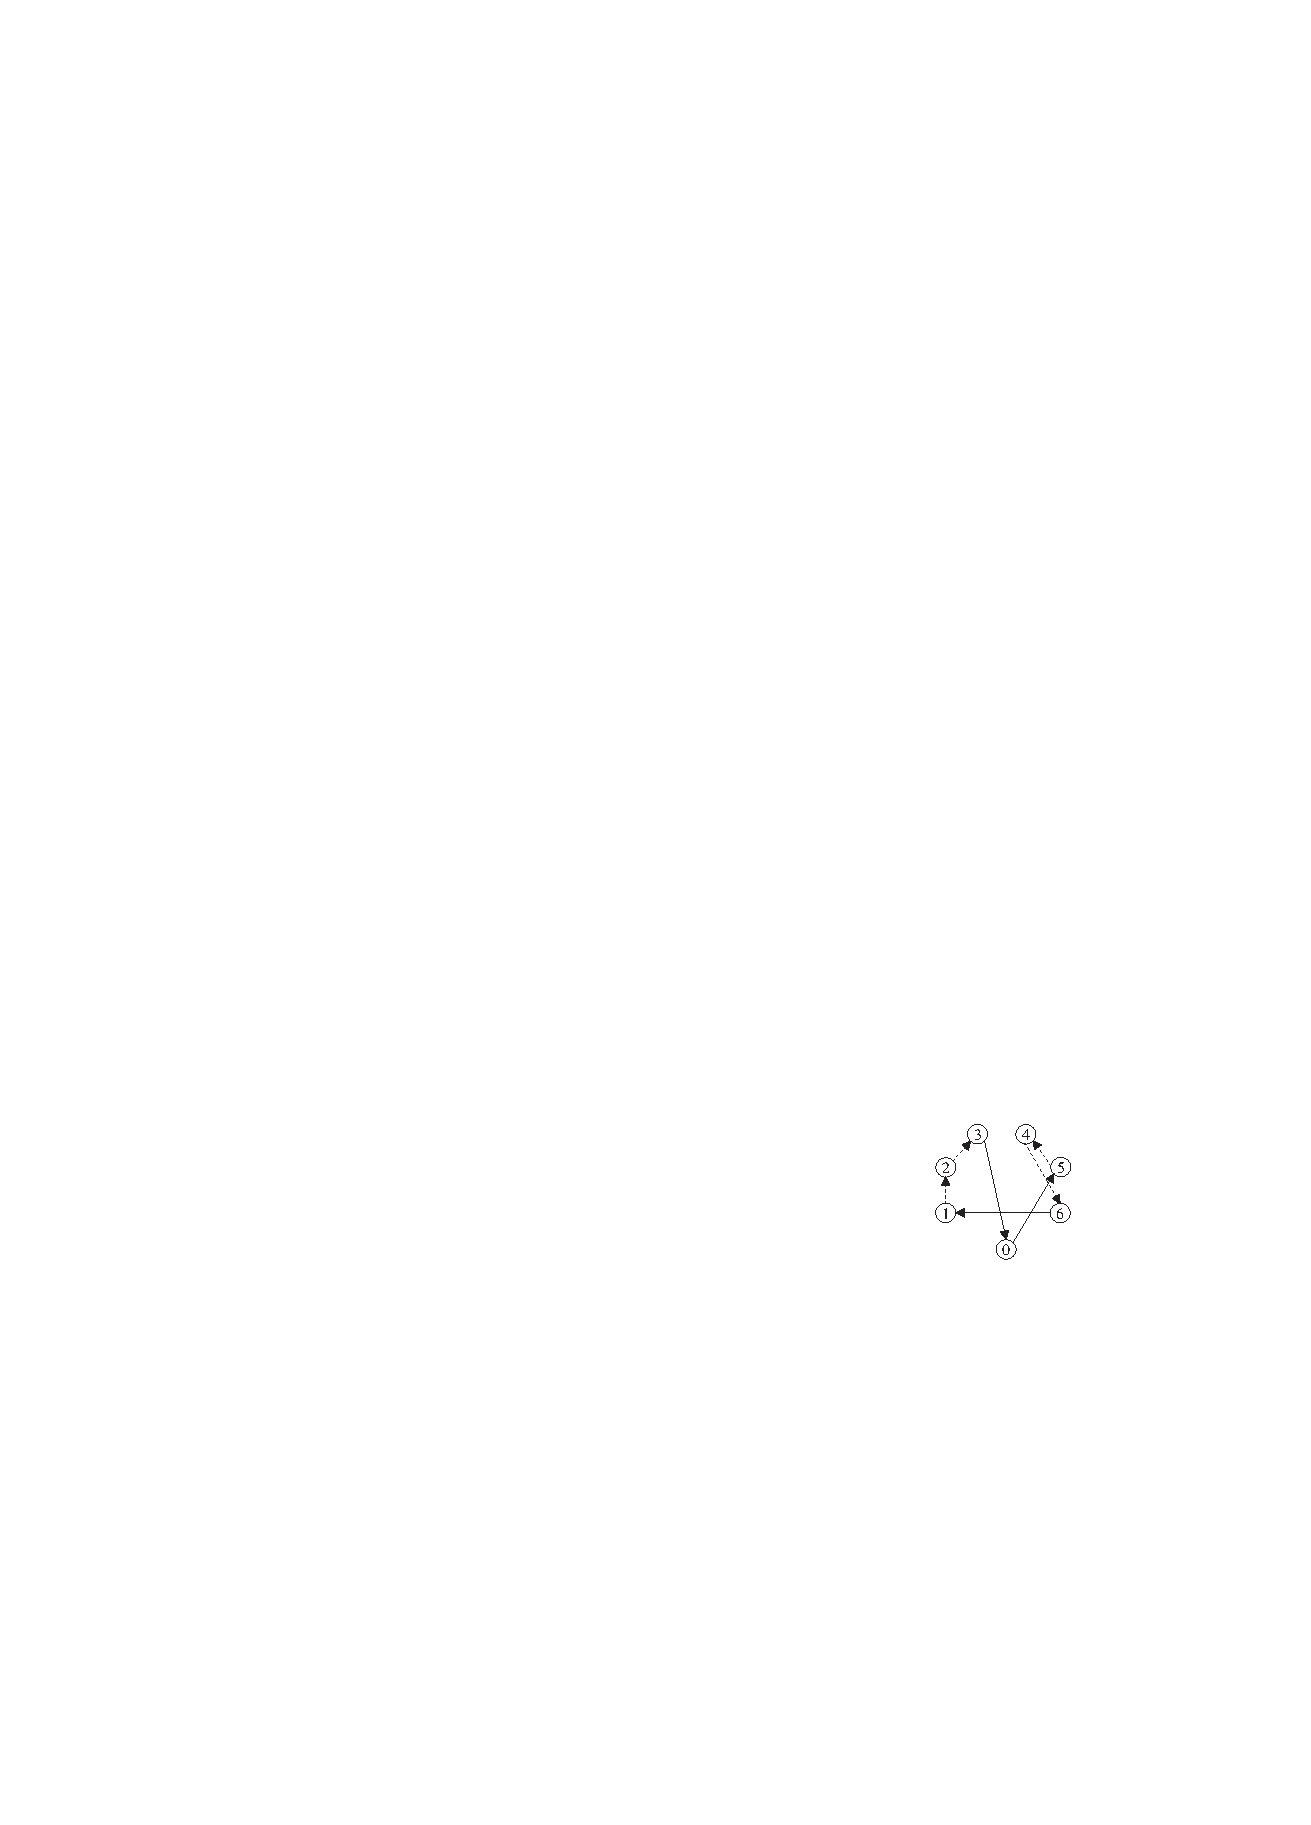
\includegraphics[height=0.75\linewidth]{image/swap.pdf}
		\caption{交换算子}
		\label{fig:swap}%文中引用该图片代号
	\end{subfigure}
	\centering
	\begin{subfigure}{0.325\linewidth}
		\centering
		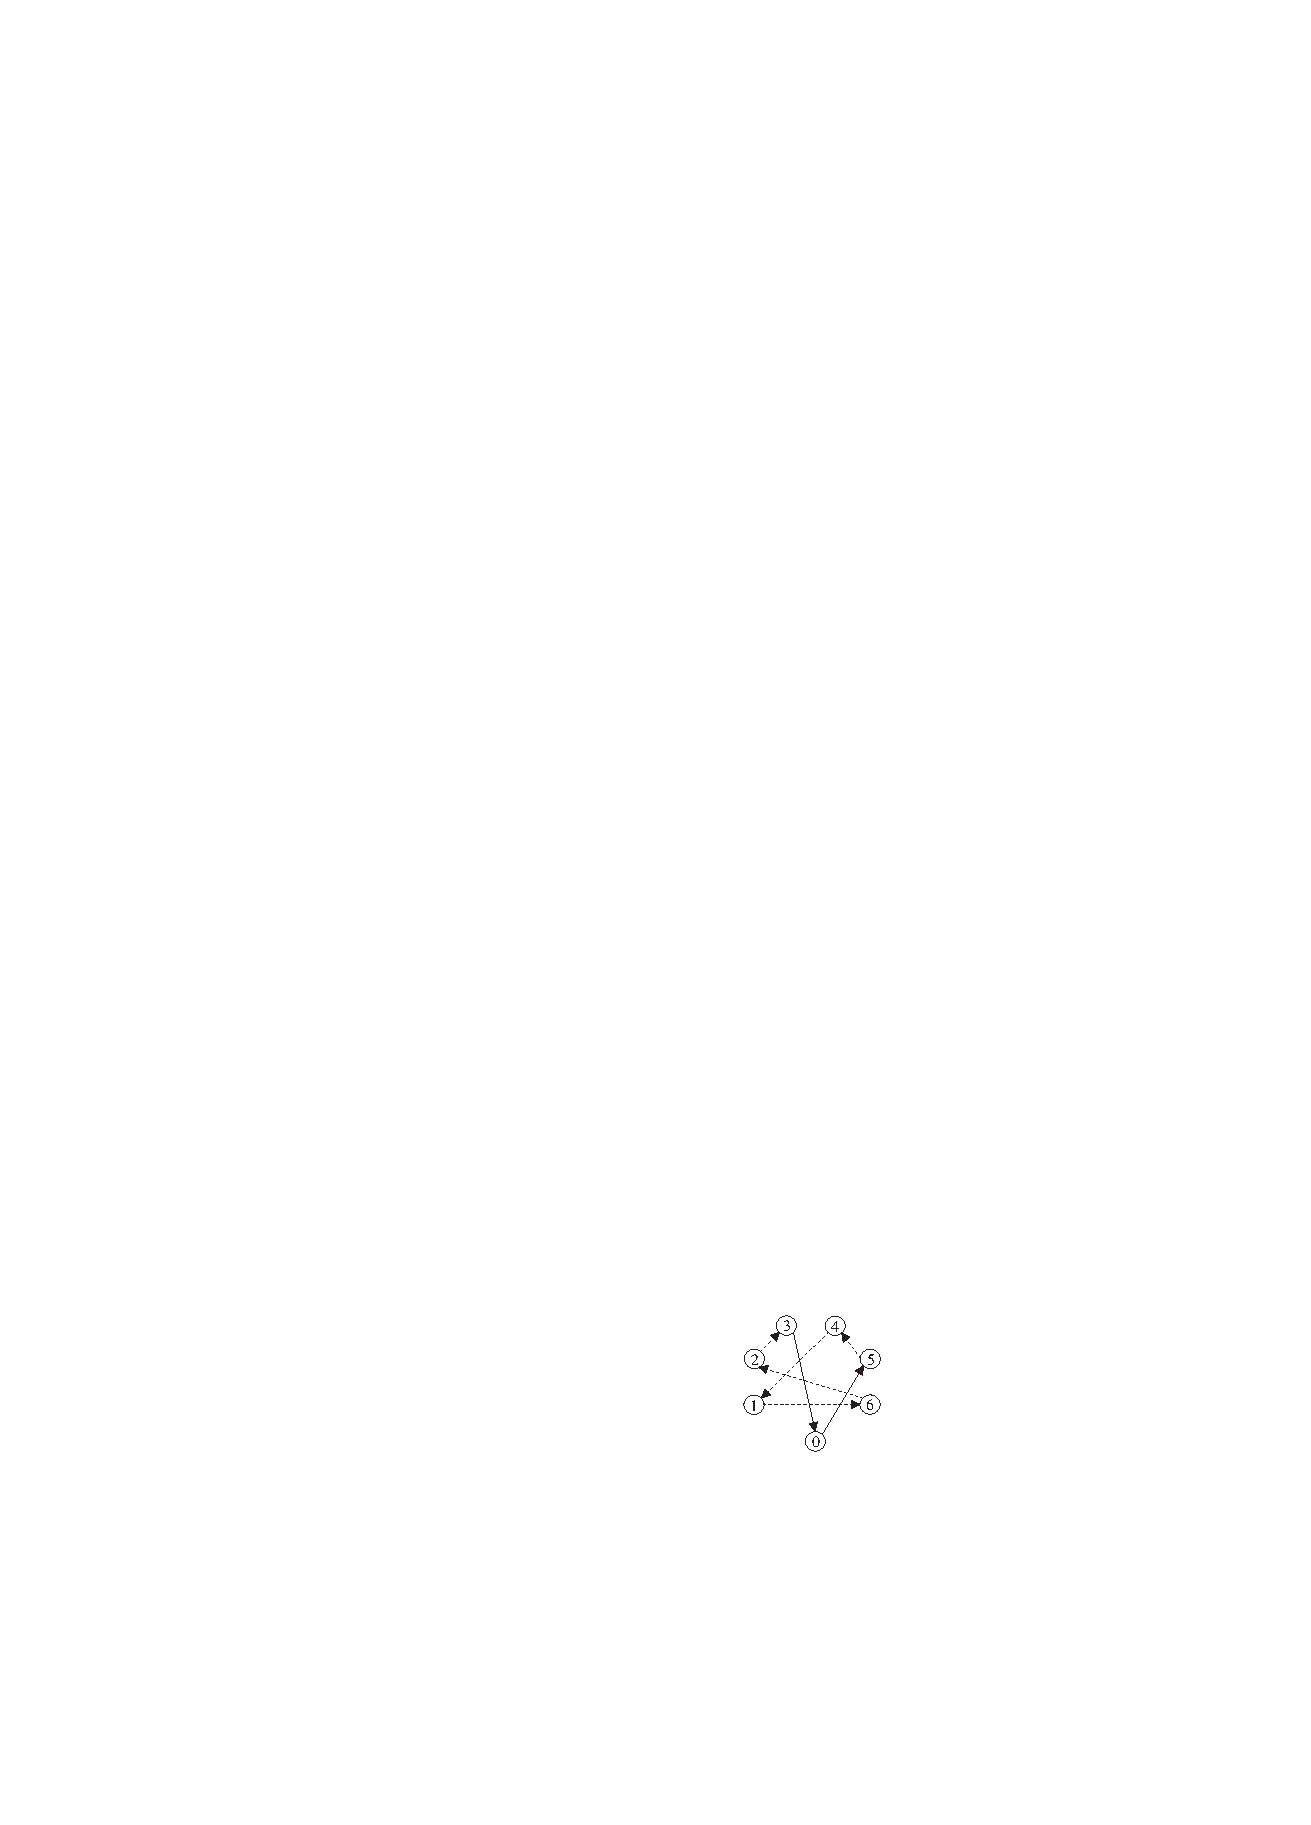
\includegraphics[height=0.75\linewidth]{image/inv.pdf}
		\caption{逆转算子}
		\label{fig:inv}%文中引用该图片代号
	\end{subfigure}
	\caption{采用的邻域算子}
	\label{fig:suanzi}
\end{figure}
随机化初始解,利用算法\ref{alg:Basic SA}计算A-n32-k5和A-n80-k10,
代码见\ref{appendix:SA},得到如\cref{tab:Basic SA32and80}、\cref{fig:A-n32-k5}
和\cref{fig:A-n80-k10}。
\begin{table}[H]
	\centering
	\caption{基本SA算法解决A-n32-k5和A-80-k10}
	\label{tab:Basic SA32and80}
	\begin{tabular}{@{}ccccccc@{}}
	\toprule
	A-n32-k5           & \texttt{SA} & \texttt{vrp} &  & A-80-k10           & \texttt{SA} & \texttt{vrp} \\ \midrule
	\texttt{num\_cars} & $10$        & $10$         &  & \texttt{num\_cars} & $10$        & $10$         \\
	\texttt{best\_obj} & $801$       & $784$        &  & \texttt{best\_obj} & $1852$      & $1764$       \\ \bottomrule
	\end{tabular}
	\end{table}
  \begin{figure}[H]
	\centering
	\begin{subfigure}{0.475\linewidth}
		\centering
		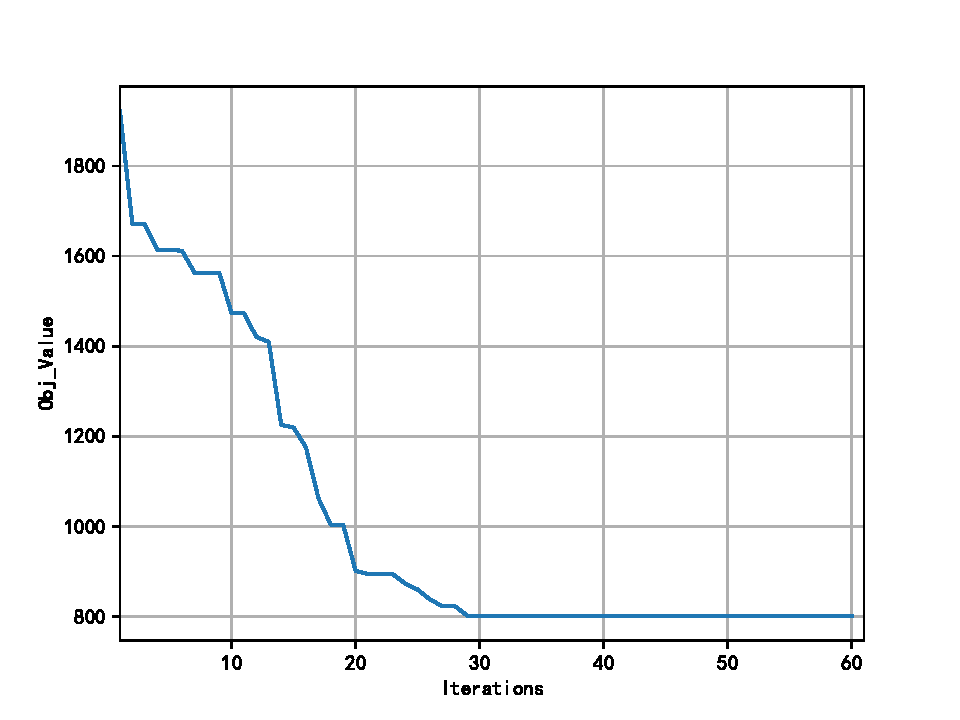
\includegraphics[height=0.85\linewidth]{image/A-n32-k5iter.pdf}
		\caption{\texttt{history\_best}-\texttt{iter}}
		\label{fig:A-n32-k5iter}%文中引用该图片代号
	\end{subfigure}
	\centering
	\begin{subfigure}{0.475\linewidth}
		\centering
		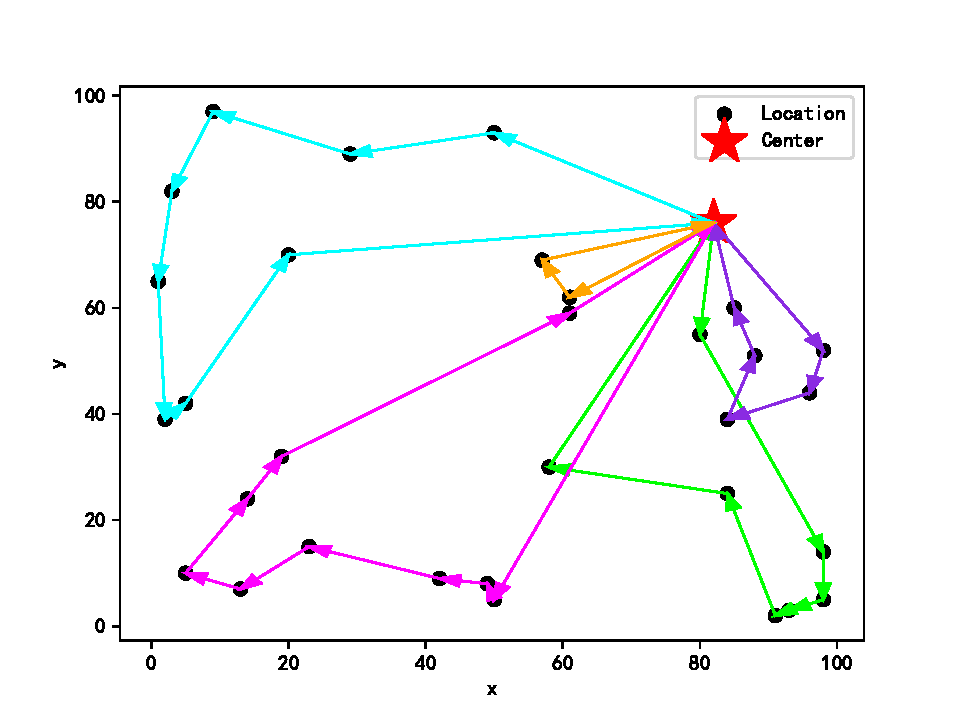
\includegraphics[height=0.85\linewidth]{image/A-n32-k5routes.pdf}
		\caption{\texttt{A-n32-k5-routes}}
		\label{fig:A-n32-k5routes}%文中引用该图片代号
	\end{subfigure}
	\caption{\texttt{A-n32-k5}运行结果}
	\label{fig:A-n32-k5}
\end{figure}
\begin{figure}[H]
	\centering
	\begin{subfigure}{0.475\linewidth}
		\centering
		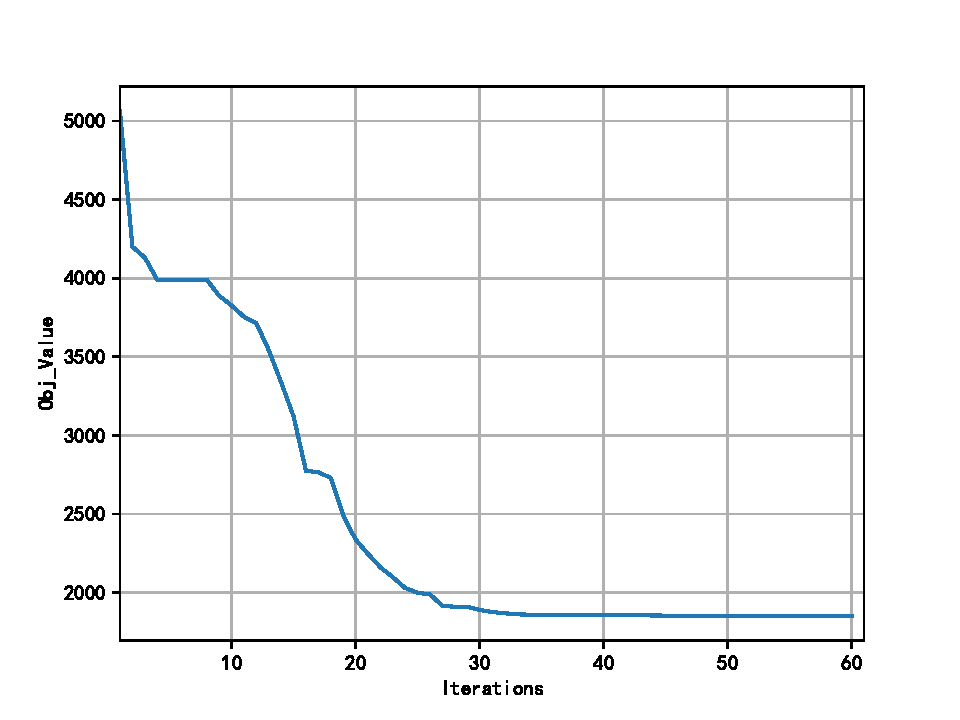
\includegraphics[height=0.85\linewidth]{image/A-n80-k10iter.pdf}
		\caption{\texttt{history\_best}-\texttt{iter}}
		\label{fig:A-n80-k10iter}%文中引用该图片代号
	\end{subfigure}
	\centering
	\begin{subfigure}{0.475\linewidth}
		\centering
		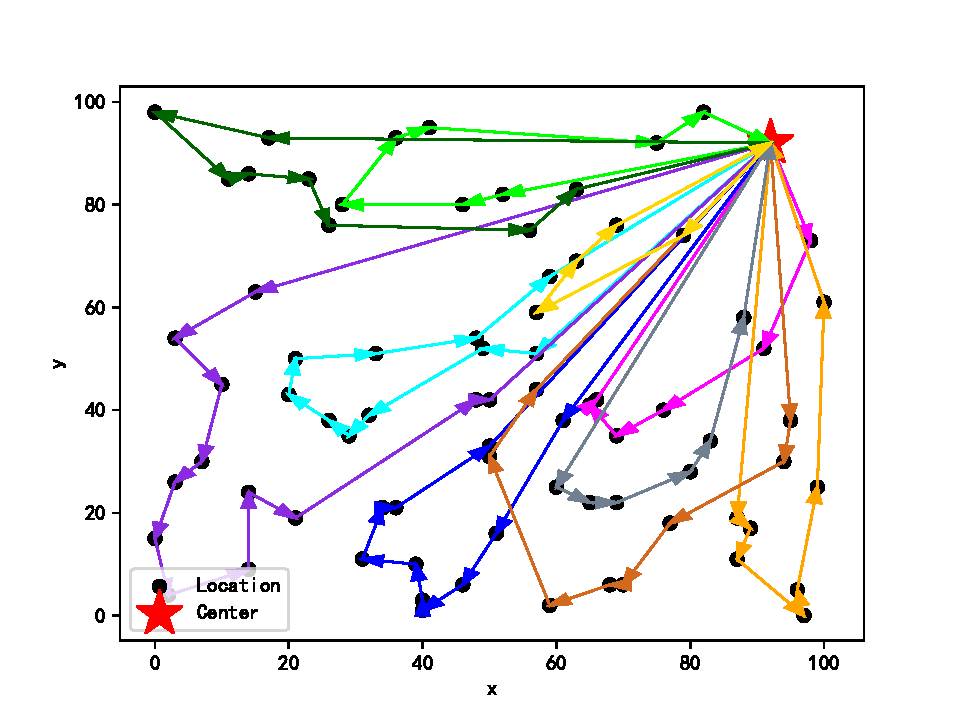
\includegraphics[height=0.85\linewidth]{image/A-n80-k10routes.pdf}
		\caption{\texttt{A-n80-k10-routes}}
		\label{fig:A-n80-k10routes}%文中引用该图片代号
	\end{subfigure}
	\caption{\texttt{A-n80-k10}运行结果}
	\label{fig:A-n80-k10}
\end{figure}
\subsection{参数优化试验}
SA 算法的参数包括初始温度$T_0$,Metropolis 抽样次数$L$
以及降温率$\alpha$,令其分别有$P_T,\, P_L$及$P_{\alpha}$种选择,则参数组合
共有$P_T\times P_L\times P_{\alpha}$种。

一种参数组合$(P_T,\, P_L,\, P_{\alpha})$为问题的一个可行解,所有的参数组合构成问题的整个解空间,大小
为$P_T\times P_L\times P_{\alpha}$。

我们在实际过程中采用了两种参数优化的策略
\begin{description}
	\item[基于经验的参数优化] 利用经验给出几组可调的参数值,遍历选取其中最好的结果。
	\item[基于贝叶斯的参数优化] 利用python集成的bayes\_opt库,得到最好的参数值。
\end{description}

\subsubsection{依据经验的参数优化}\label{subsubsec:exp}
选择参数如\cref{eq:experience}:
\begin{equation}\label{eq:experience}
\left\{
	\begin{array}{cl}
	T_0 =& \{50, 100, 200, 300, 500\} \\
	\alpha =& \{0.8, 0.85 ,0.9, 0.95\} \\
	num_{Tk} =& \{1, 2, 3, 4, 5 ,6, 7\} 	
	\end{array}
\right.
\end{equation}
其中抽样次数$L$为邻域大小的倍数$\mathtt{len}(actionlist) \times num_{Tk}$。
如果要串行运算所有可能的情况,需要$5\times 4\times 7 = 140$次,故而我们将其可能的参数
组合划分,并行计算,代码如\ref{appendix:bingxing}。

得到的较优的结果的参数组合为\cref{tab:experience},
\begin{table}[htbp]
	\centering
	\caption{经验参数优化}
	  \begin{tabular}{ccccccccc}
	  \toprule
	  $ T_0$ & $\alpha $ & $num_{Tk}$ & A-n32-k5的结果 &     & $ T_0$ & $\alpha $ & $num_{Tk}$ & A-n32-k5的结果 \\
	  \midrule
	  300 & 0.8 & 1   & 797.45129 &     & 200 & 0.8 & 6   & 797.4513 \\
	  300 & 0.8 & 4   & 797.45129 &     & 200 & 0.9 & 4   & 797.4513 \\
	  500 & 0.85 & 7   & 797.45129 &     & 50  & 0.8 & 6   & 798.9434 \\
	  200 & 0.85 & 2   & 797.45129 &     & 100 & 0.85 & 2   & 798.9434 \\
	  \bottomrule
	  \end{tabular}%
	\label{tab:experience}%
\end{table}%
选取\cref{tab:experience}中不同参数组合测试所有vrp问题数据,得到\cref{fig:exp}。
\begin{figure}[H]
	\centering
	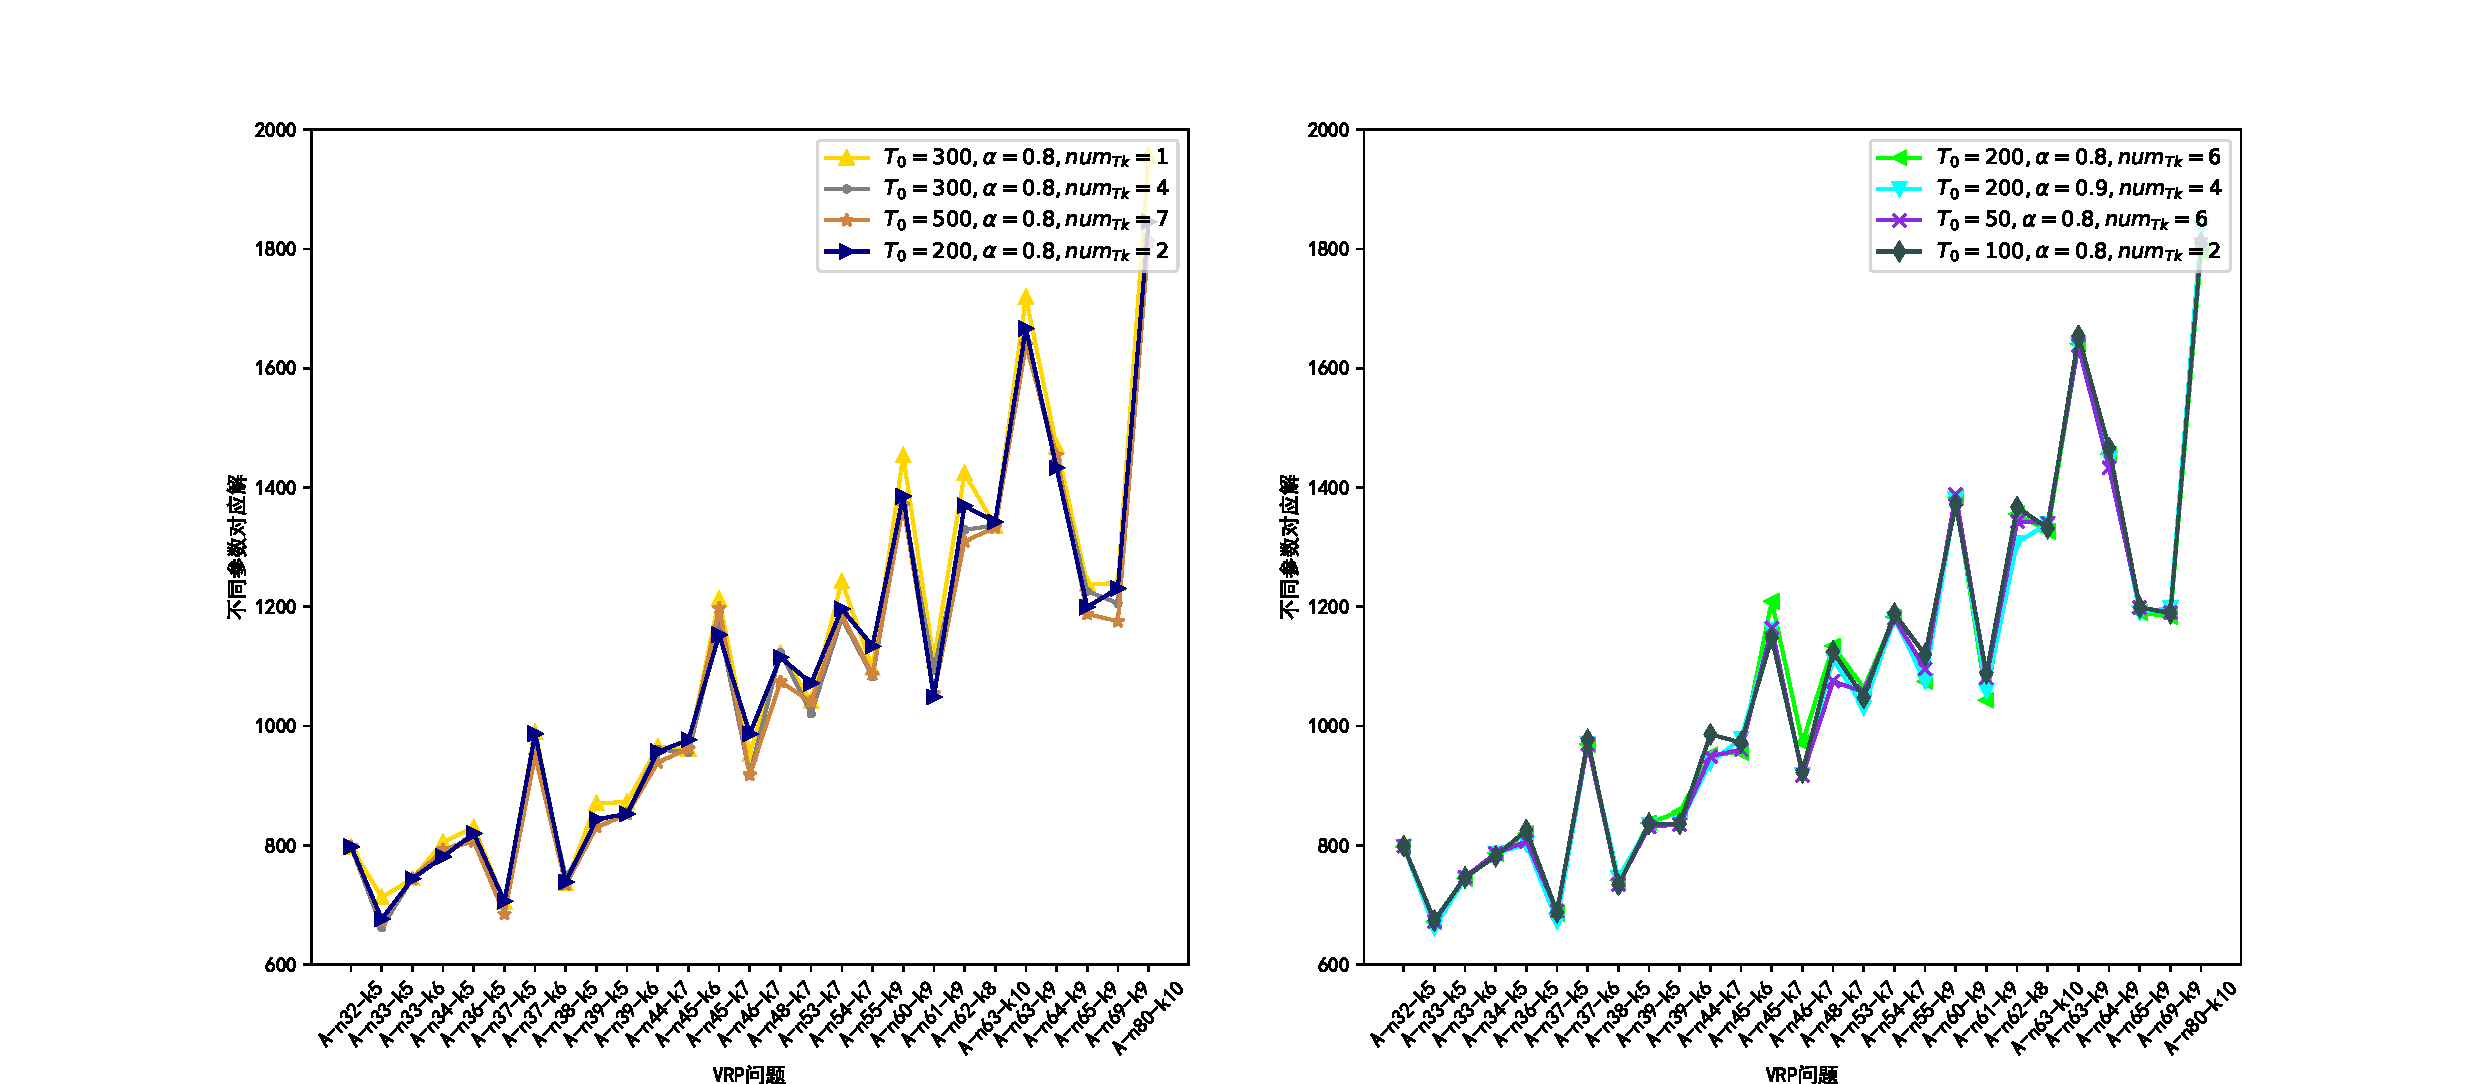
\includegraphics[width=\textwidth]{image/exp.pdf}
	\caption{较优的几组经验参数对应vrp的解}	
	\label{fig:exp}
\end{figure} 
  
\subsubsection{依据贝叶斯的参数优化}\label{subsubsec:bayes}
由于SA算法本身存在随机因素,因此也可以将算法参数设定问题视为
随机组合优化问题。这类问题往往不知道自变量与因变量的关系,
但是只知道最后函数大概什么走向(也就是自变量对因变量大概的影响)。

而贝叶斯优化的好处在于只需要不断取样\cite{2020Surrogates},来推测函数的最大值。并且采样的点也不多。
因此,模拟退火算法(SA)的参数设定非常适合利用贝叶斯优化的方法。

具体思路如下:

由于我们要优化的这个函数计算量太大,一个自然的想法就是用一个简单点的模型来近似,
这个替代原始函数的模型也叫做代理模型,贝叶斯优化中的代理模型为\textbf{高斯过程}。
假设我们对待优化函数的先验(prior)为高斯过程,
经过一定的试验我们有了数据(也就是evidence),
然后根据贝叶斯定理就可以得到这个函数的后验分布。

有了这个后验分布后,我们需要考虑下一次试验点在哪里进一步收集数据,
因此就会需要构造一个acquisition函数用于指导搜索方向(选择下一个试验点),
然后再去进行试验,得到数据后更新代理模型的后验分布,反复进行。

综上所述,贝叶斯优化的流程为:
\begin{algorithm}[H]
	\caption{贝叶斯优化流程}  
	\label{alg:Bayes Opt}
	\begin{algorithmic}[1] %每行显示行号  
		\Require 迭代次数$max\_iter=30$, 初始抽样点数$init\_points=5$
		\Ensure 最优解对应参数$\mathbf{x}$,最优解$\min\ z $
		\Procedure{Bayesian Optimization}{ $max\_iter=30, init\_points=5$ }
				\For{ $t = 1 \to max\_iter$ } 
					\State Find $x_{t}$ by \textbf{optimizing the acquisition function} over the GP:
					$\mathbf{x}_t = \mathop{\arg\min}\limits_{\mathbf{x}}\ u(\mathbf{x}|D_{1:t-1})$
					\State \textbf{Sample} the objective function:$y_t = f(\mathbf{x}_t)+\varepsilon_t$ 
					\State Augment the data and update the GP:$D_{1:t} = \{ D_{1:t-1},(\mathbf{x}_t;y_t) \}$ and update the GP
				\EndFor 
		\EndProcedure  
	\end{algorithmic}  
\end{algorithm} 
高斯过程和acquisition函数见\ref{appendix:guess}。

选择初始抽样点数目为5,迭代次数为30次,按照距离从小到大排序,挑选
较好的结果如\cref{tab:Bayes},代码见\ref{appendix:bayos}。
\begin{table}[htbp]
	\centering
	\caption{贝叶斯的参数优化}
	  \begin{tabular}{ccccccccccc}
	  \toprule
	  iter & target & $T_{0}$ & $\alpha$ & $num_{Tk}$ &     & iter & target & $T_{0}$ & $\alpha$ & $num_{Tk}$ \\
	  \midrule
	  34  & 797.4482 & 85.34 & 0.9237 & 1.506 &     & 22  & 804.5052 & 47.63 & 0.9173 & 5.801 \\
	  21  & 798.0846 & 29.35 & 0.8012 & 2.342 &     & 13  & 805.153 & 43.91 & 0.7872 & 4.06 \\
	  16  & 801.2821 & 41.19 & 0.8072 & 3.08 &     & 26  & 805.153 & 20.51 & 0.8309 & 2.868 \\
	  20  & 801.9246 & 36.39 & 0.9185 & 4.715 &     & 31  & 806.4516 & 43.55 & 0.8832 & 1.998 \\
	  10  & 803.2129 & 27.1 & 0.86 & 4.974 &     & 35  & 807.7544 & 22.37 & 0.8769 & 5.267 \\
	  14  & 803.2129 & 94.34 & 0.9004 & 4.89 &     & 23  & 808.4074 & 94.02 & 0.8189 & 2.402 \\
	  3   & 803.8585 & 77.96 & 0.912 & 1.362 &     &     &     &     &     &  \\
	  \bottomrule
	  \end{tabular}%
	\label{tab:Bayes}%
  \end{table}%

  选取\cref{tab:Bayes}中不同参数组合测试所有vrp问题数据,得到\cref{fig:bayes_opt}。
\begin{figure}[H]
	\centering
	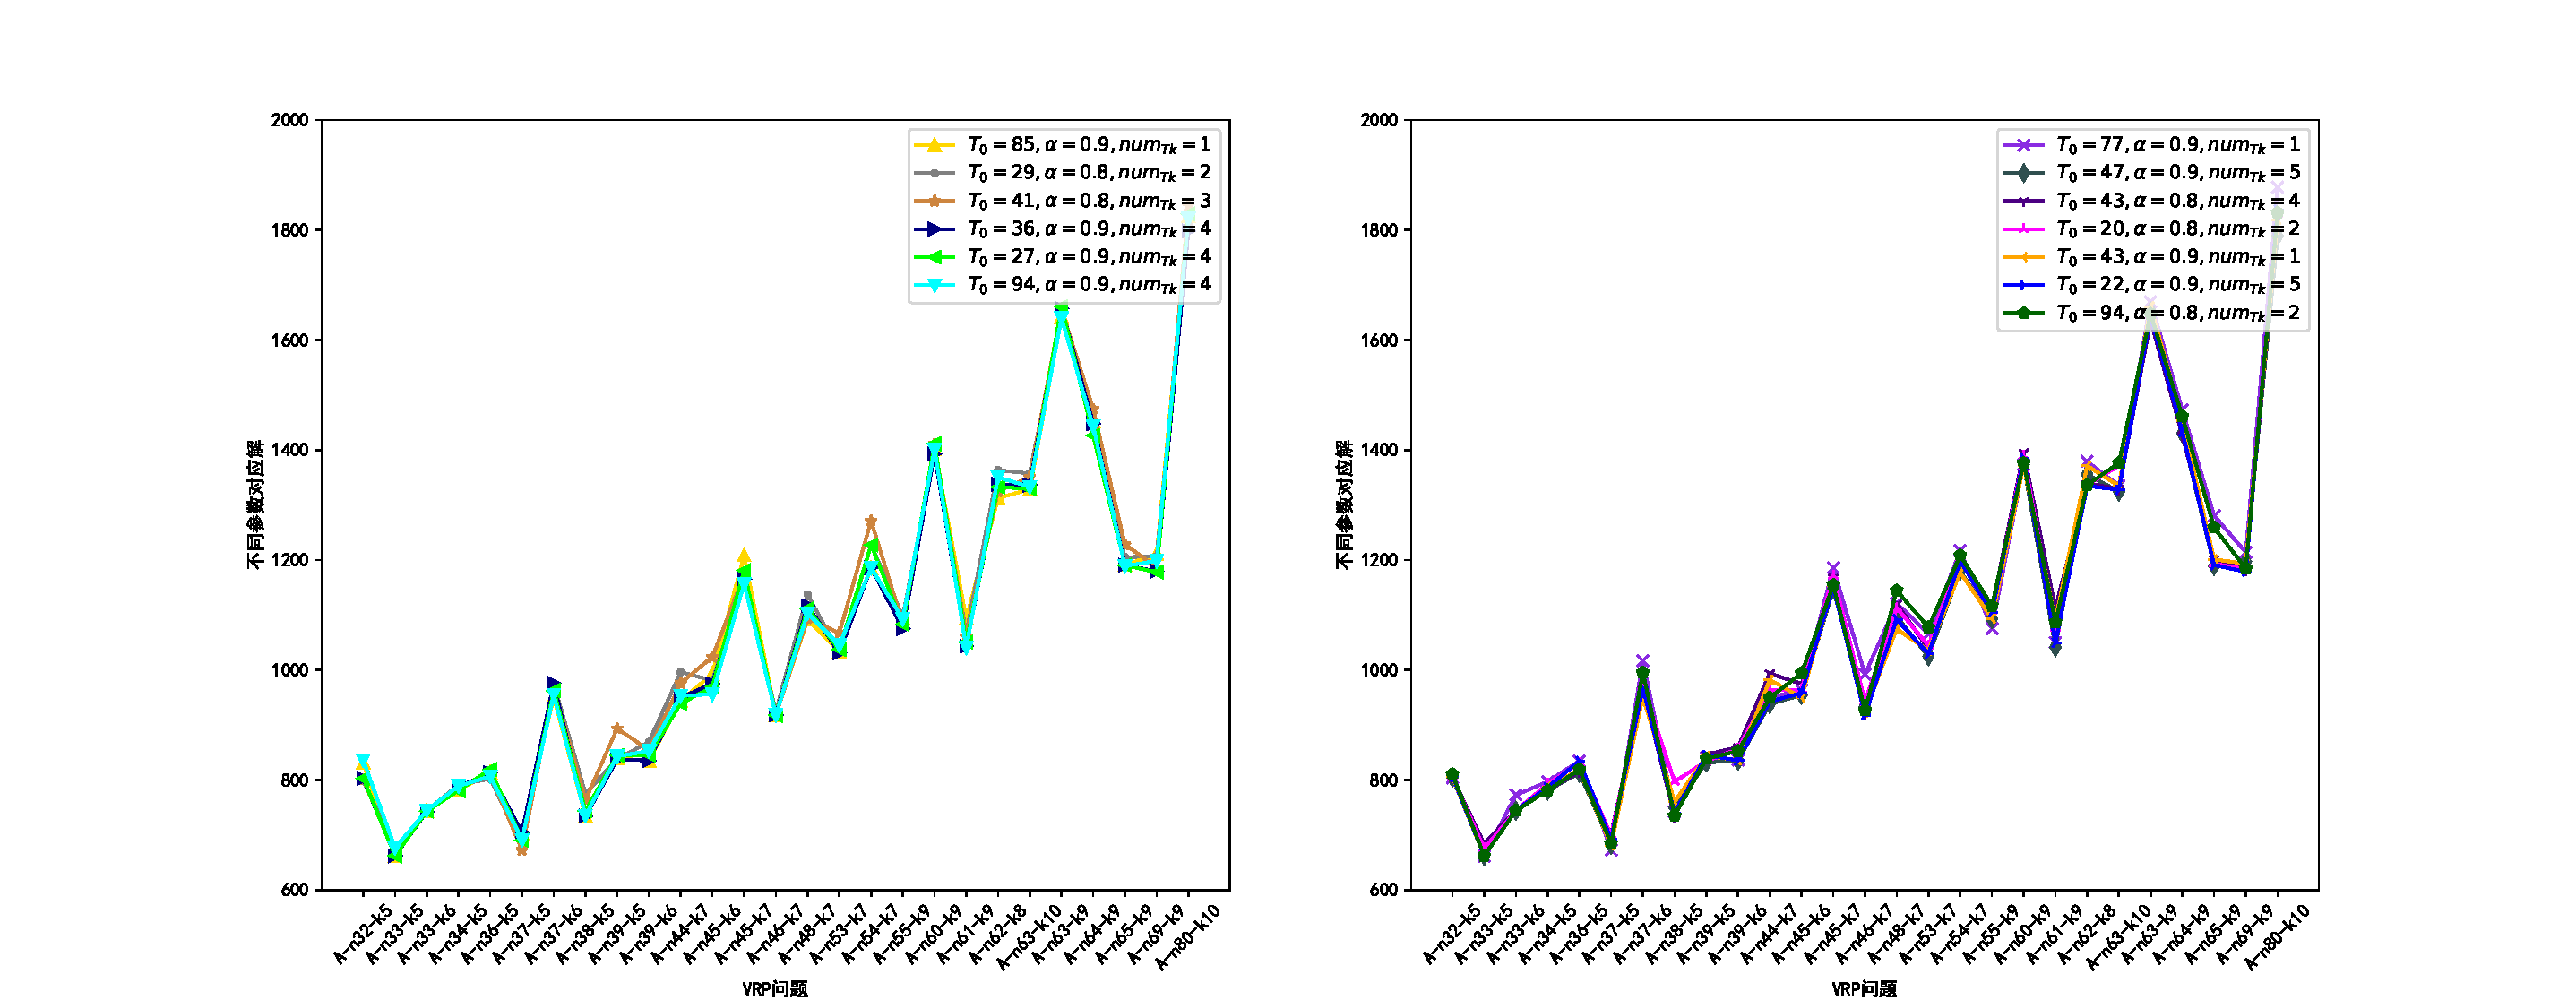
\includegraphics[width=\textwidth]{image/Bayes opt.pdf}
	\caption{较优的几组贝叶斯优化参数对应vrp的解}
	\label{fig:bayes_opt}
\end{figure}
\subsection{实验结果}
计算依据\ref{subsubsec:exp}节和\ref{subsubsec:bayes}节得到的
所有第$i$组参数对应的最优解$opt_{ij}$与vrp问题现已知最优解$opt\_now_{ij}$的差值之和
\[
	minus = \sum\limits_{j = 1}^{N}	opt_{ij}-opt\_now_{ij}
\]
我们所求的最优参数组合为
\[
	\mathbf{x} = \mathop{\arg\min}\limits_{\mathbf{x}}\ minus=\mathop{\arg\min}\limits_{\mathbf{x}}\ \sum\limits_{j = 1}^{N}(opt_{ij}-opt\_now_{ij})
\]
由上选取的最优组合如\cref{tab:exp and bayes index}:
\begin{table}[htbp]
	\centering
	\caption{两种参数优化结果}
	  \begin{tabular}{cccccc}
	  \toprule
		  & $ T_0$ & $\alpha $ & $num_{Tk}$ & 所有路径总和 & 已经得到的的最优解 \\
	  \midrule
	  经验参数 & 500 & 0.85 & 7   & 28609.29953 & \multirow{2}[2]{*}{28222} \\
	  贝叶斯优化参数 & 47.63 & 0.9173 & 5.801 & 28582.5199 &  \\
	  \bottomrule
	  \end{tabular}%
	\label{tab:exp and bayes index}%
  \end{table}%

可以看出贝叶斯优化的参数整体更优,但是总的距离分担到每一个vrp问题
其实差距不大。
\begin{table}[htbp]
	\centering
	\caption{经验参数$T_0=500,\ \alpha=0.85,\ num_{Tk}=7$的VRP问题距离}
	  \begin{tabular}{ccccccccccc}
	  \toprule
	  \textbf{x\_list} & \textbf{y} &     & \textbf{x\_list} & \textbf{y} &     & \textbf{x\_list} & \textbf{y} &     & \textbf{x\_list} & \textbf{y} \\
	  \midrule
	  A-n32-k5 & 797.4513 &     & A-n38-k5 & 734.1847 &     & A-n48-k7 & 1074.338 &     & A-n63-k10 & 1333.255 \\
	  A-n33-k5 & 674.1165 &     & A-n39-k5 & 830.7456 &     & A-n53-k7 & 1040.617 &     & A-n63-k9 & 1639.088 \\
	  A-n33-k6 & 744.2418 &     & A-n39-k6 & 852.6008 &     & A-n54-k7 & 1186.567 &     & A-n64-k9 & 1454.067 \\
	  A-n34-k5 & 792.5381 &     & A-n44-k7 & 939.2543 &     & A-n55-k9 & 1086.692 &     & A-n65-k9 & 1187.933 \\
	  A-n36-k5 & 806.7829 &     & A-n45-k6 & 962.2644 &     & A-n60-k9 & 1369.716 &     & A-n69-k9 & 1175.815 \\
	  A-n37-k5 & 684.9976 &     & A-n45-k7 & 1197.484 &     & A-n61-k9 & 1054.617 &     & A-n80-k10 & 1811.23 \\
	  A-n37-k6 & 950.8523 &     & A-n46-k7 & 918.2779 &     & A-n62-k8 & 1309.574 &     &     &  \\
	  \bottomrule
	  \end{tabular}%
	\label{tab:exp_index}%
  \end{table}%
\begin{table}[htbp]
	\centering
	\caption{贝叶斯优化参数$T_0=47.63,\ \alpha=0.9173,\ num_{Tk}=5.801$}
	  \begin{tabular}{ccccccccccc}
	  \toprule
	  \textbf{x\_list} & \textbf{y} &     & \textbf{x\_list} & \textbf{y} &     & \textbf{x\_list} & \textbf{y} &     & \textbf{x\_list} & \textbf{y} \\
	  \midrule
	  A-n32-k5 & 804.7916 &     & A-n38-k5 & 749.889 &     & A-n48-k7 & 1097.042 &     & A-n63-k10 & 1324.492 \\
	  A-n33-k5 & 662.1101 &     & A-n39-k5 & 831.6498 &     & A-n53-k7 & 1024.978 &     & A-n63-k9 & 1652.328 \\
	  A-n33-k6 & 744.2418 &     & A-n39-k6 & 835.2518 &     & A-n54-k7 & 1180.096 &     & A-n64-k9 & 1430.108 \\
	  A-n34-k5 & 780.9361 &     & A-n44-k7 & 938.1813 &     & A-n55-k9 & 1092.752 &     & A-n65-k9 & 1189.281 \\
	  A-n36-k5 & 812.9845 &     & A-n45-k6 & 954.4739 &     & A-n60-k9 & 1373.748 &     & A-n69-k9 & 1196.691 \\
	  A-n37-k5 & 682.3335 &     & A-n45-k7 & 1146.909 &     & A-n61-k9 & 1041.58 &     & A-n80-k10 & 1788.94 \\
	  A-n37-k6 & 956.8075 &     & A-n46-k7 & 934.2195 &     & A-n62-k8 & 1355.704 &     &     &  \\
	  \bottomrule
	  \end{tabular}%
	\label{tab:bayes_index}%
  \end{table}%
	
运行得到的结果如\cref{fig:exp and bayes index},
每一个vrp问题对应的路径长度如\cref{tab:exp_index}
和\cref{tab:bayes_index},每一个VRP问题的路径
见\ref{appendix:bayesVRP}。

\begin{figure}[htbp]
	\centering
	\begin{subfigure}{0.467\linewidth}
		\centering
		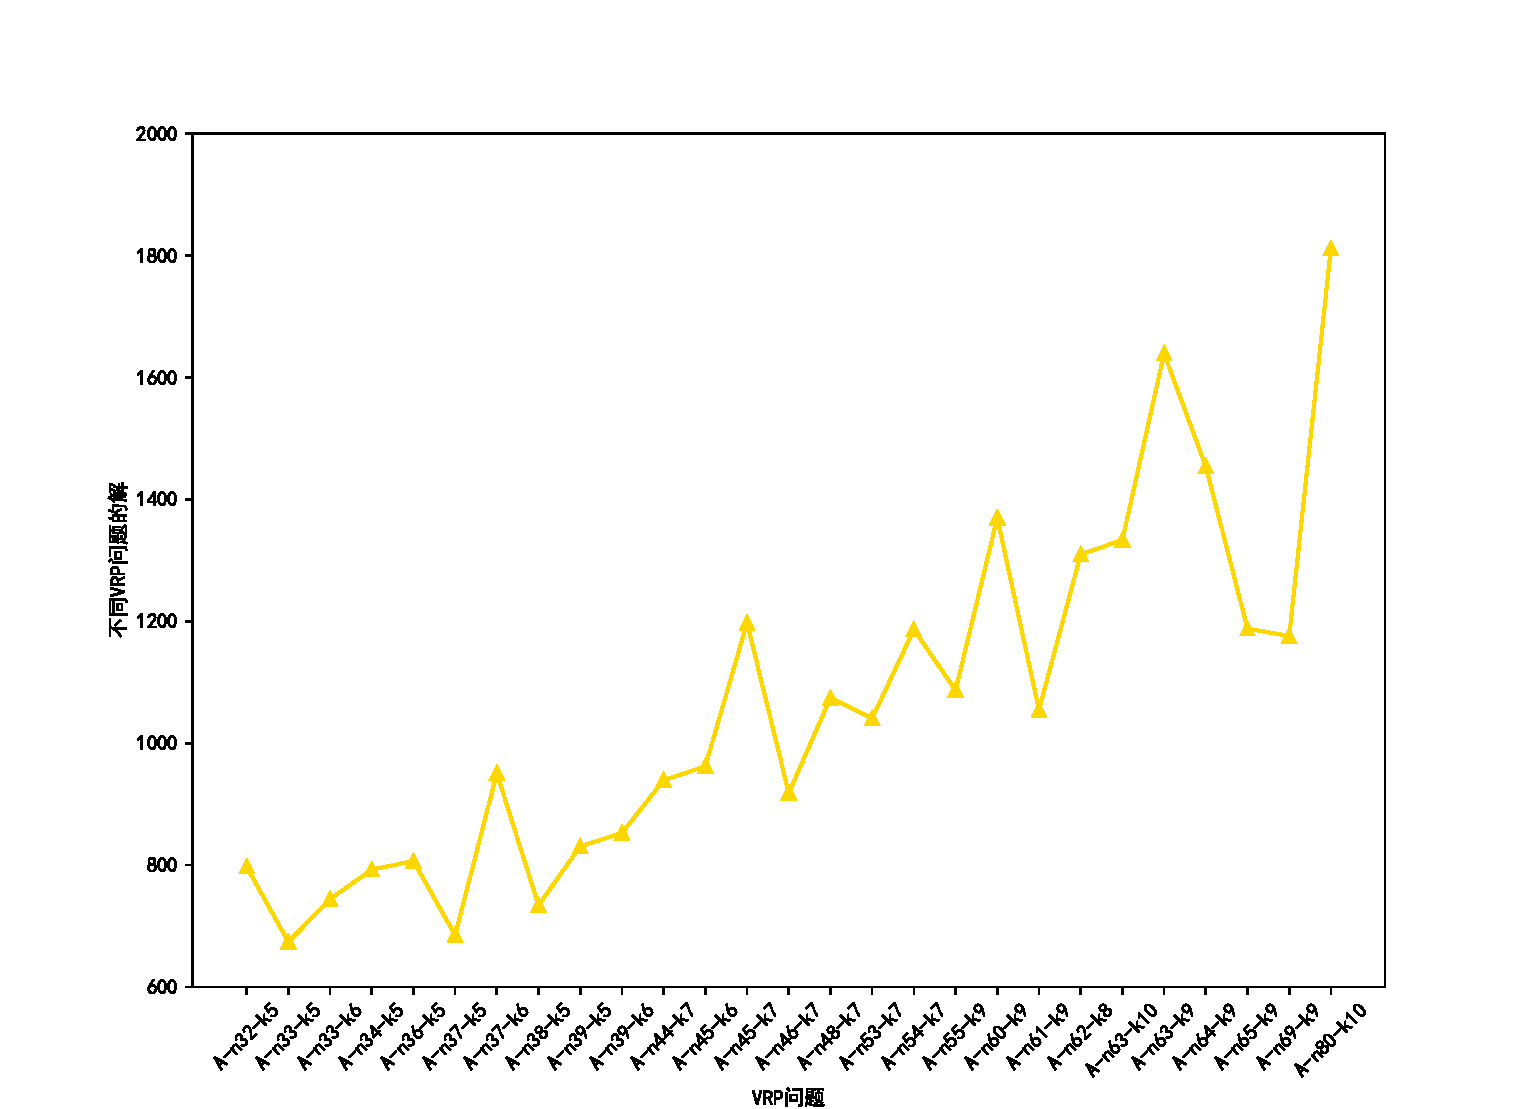
\includegraphics[height=0.85\linewidth]{image/exp_best.pdf}
		\caption{最优经验参数对应解}
		\label{fig:exp_best}%文中引用该图片代号
	\end{subfigure}
	\hspace*{17pt}
	\centering
	\begin{subfigure}{0.475\linewidth}
		\centering
		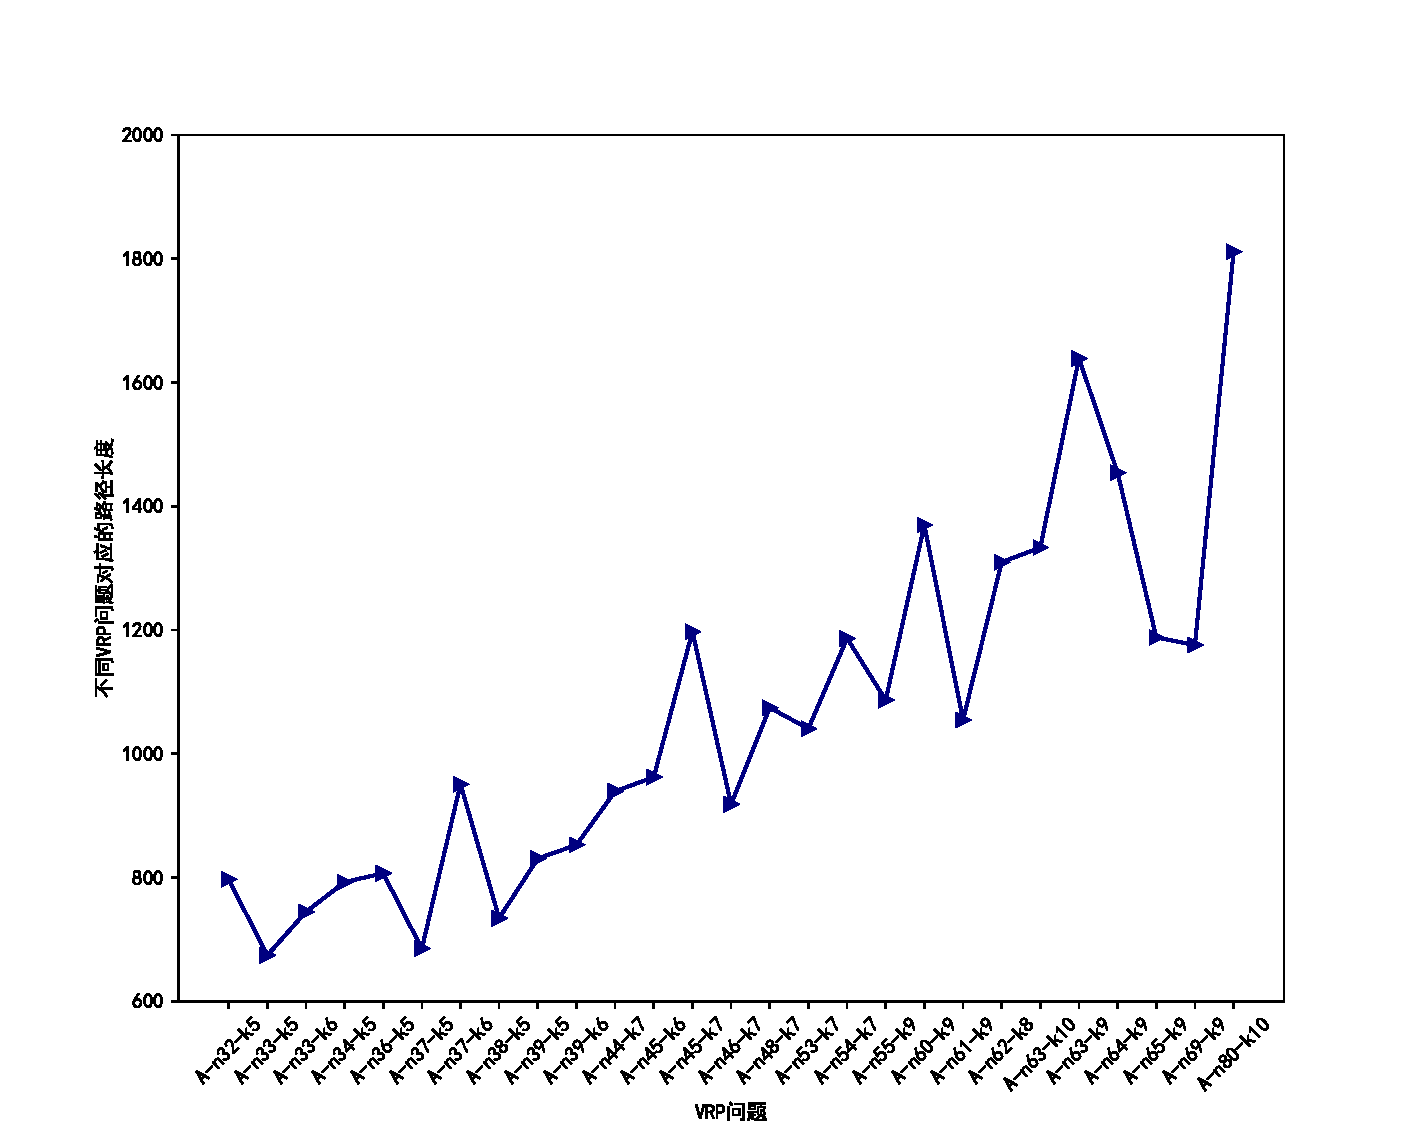
\includegraphics[height=0.85\linewidth]{image/bayes_best.pdf}
		\caption{最优贝叶斯参数对应解}
		\label{fig:bayes_best}%文中引用该图片代号
	\end{subfigure}
	\caption{两种最优参数对应解}
	\label{fig:exp and bayes index}
\end{figure}

\section{改进的模拟退火算法}
\subsection{添加每条路径TSP优化的改进} 
我们构造的解是符合容量限制的,但是每一条路径对应的TSP问题并不一定
是最短的,故而对与每一条路径的优化是我们改进的重要方向之一。

因为每一辆车走过的路径点数比较少,我们选择利用分支定界法
求得每一辆车对应TSP问题的最优解来改进总的VRP问题。
但是我们发现,在参数改进后,每条路径的TSP都已经是最优解了,方法改进作用不大。

\subsection{减小最大迭代次数的改进}
如\cref{fig:A-n32-k5iter}和\cref{fig:A-n80-k10iter},
可以看出在只设置终止温度、不设置最大迭代次数情况下,
只需要一半的迭代次数就收敛了。

故而,为了减少运行时间,最好设置最大迭代次数,在已经到达算法能达到
的最优解时就停止降温。
将最大迭代次数$max\_iter$设置为所有VRP问题中需要迭代次数最长的
收敛的次数,减少运行时间的同时保证收敛到当前的最优解。

运行时长如\cref{tab:timeimprove}和\cref{tab:timenoim}:
% Table generated by Excel2LaTeX from sheet 'Sheet1'
\begin{table}[H]
	\centering
	\caption{$max\_iter=60$的运行花费时间}
	  \begin{tabular}{ccccccccccc}
	  \toprule
	  \textbf{VRP问题} & \textbf{time} &     & \textbf{VRP问题} & \textbf{time} &     & \textbf{VRP问题} & \textbf{time} &     & \textbf{VRP问题} & \textbf{time} \\
	  \midrule
	  A-n32-k5 & 7.21 &     & A-n38-k5 & 12.61 &     & A-n48-k7 & 26.04 &     & A-n63-k10 & 54.12 \\
	  A-n33-k5 & 8.35 &     & A-n39-k5 & 14.24 &     & A-n53-k7 & 33.33 &     & A-n63-k9 & 48.25 \\
	  A-n33-k6 & 8.15 &     & A-n39-k6 & 12.93 &     & A-n54-k7 & 34.90 &     & A-n64-k9 & 55.93 \\
	  A-n34-k5 & 8.36 &     & A-n44-k7 & 20.17 &     & A-n55-k9 & 34.13 &     & A-n65-k9 & 56.61 \\
	  A-n36-k5 & 10.63 &     & A-n45-k6 & 20.36 &     & A-n60-k9 & 44.54 &     & A-n69-k9 & 61.42 \\
	  A-n37-k5 & 11.46 &     & A-n45-k7 & 21.13 &     & A-n61-k9 & 51.47 &     & A-n80-k10 & 92.57 \\
	  A-n37-k6 & 12.33 &     & A-n46-k7 & 23.17 &     & A-n62-k8 & 43.62 &     &     &  \\
	  \bottomrule
	  \end{tabular}%
	\label{tab:timeimprove}%
  \end{table}%
% Table generated by Excel2LaTeX from sheet 'Sheet1'
\begin{table}[H]
	\centering
	\caption{不设置迭代次数的运行时间}
	  \begin{tabular}{ccccccccccc}
	  \toprule
	  \textbf{VRP问题} & \textbf{time} &     & \textbf{VRP问题} & \textbf{time} &     & \textbf{VRP问题} & \textbf{time} &     & \textbf{VRP问题} & \textbf{time} \\
	  \midrule
	  A-n32-k5 & 13.22 &     & A-n38-k5 & 24.39 &     & A-n48-k7 & 45.06 &     & A-n63-k10 & 96.18 \\
	  A-n33-k5 & 15.66 &     & A-n39-k5 & 25.10 &     & A-n53-k7 & 59.58 &     & A-n63-k9 & 93.43 \\
	  A-n33-k6 & 15.50 &     & A-n39-k6 & 24.79 &     & A-n54-k7 & 63.41 &     & A-n64-k9 & 98.69 \\
	  A-n34-k5 & 16.77 &     & A-n44-k7 & 36.79 &     & A-n55-k9 & 68.16 &     & A-n65-k9 & 109.26 \\
	  A-n36-k5 & 20.55 &     & A-n45-k6 & 37.57 &     & A-n60-k9 & 81.15 &     & A-n69-k9 & 135.42 \\
	  A-n37-k5 & 20.99 &     & A-n45-k7 & 39.07 &     & A-n61-k9 & 87.31 &     & A-n80-k10 & 203.49 \\
	  A-n37-k6 & 22.97 &     & A-n46-k7 & 40.89 &     & A-n62-k8 & 85.86 &     &     &  \\
	  \bottomrule
	  \end{tabular}%
	\label{tab:timenoim}%
  \end{table}%
二者对比如\cref{fig:withorno_max_iter},可见在增加最大迭代次数的限制后
运行时间几乎缩短了一半。
\begin{figure}[H]
	\centering
	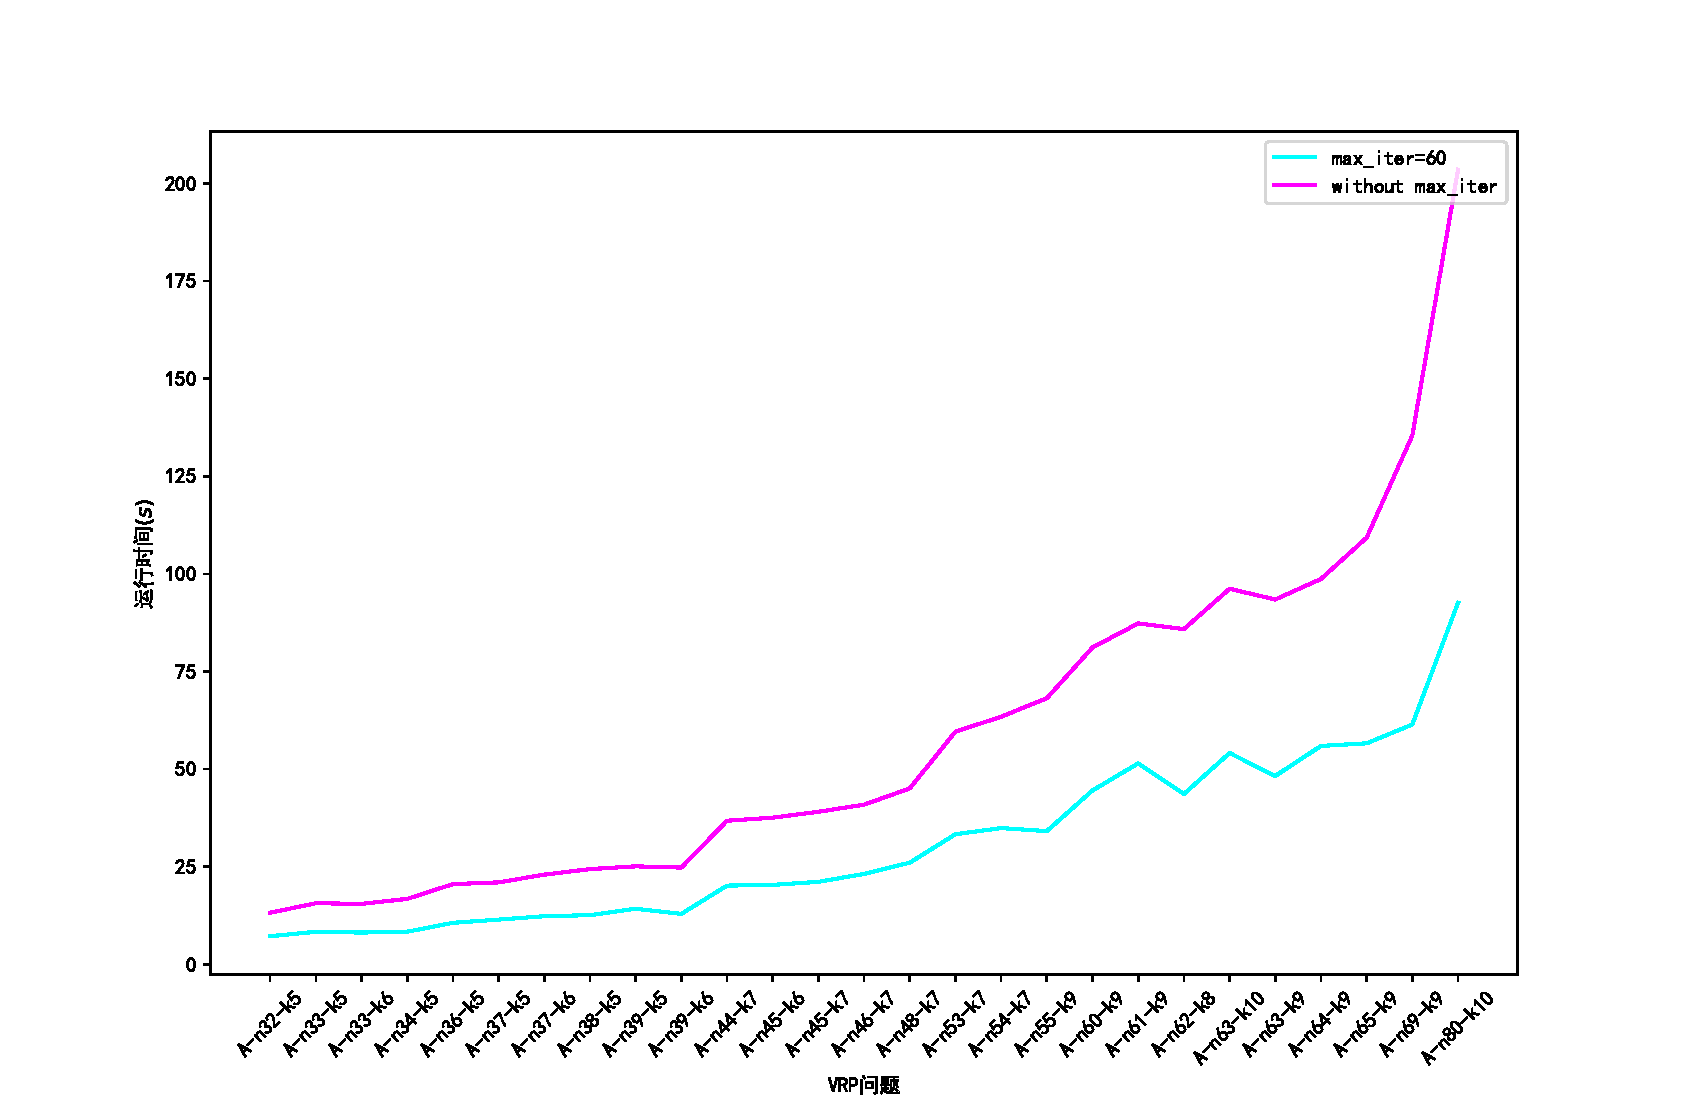
\includegraphics[height = 0.45\linewidth]{image/time_contrast.pdf}
	\caption{有无最大迭代次数$max\_iter$}
	\label{fig:withorno_max_iter}
\end{figure}

\newpage
\nocite{*}
\printbibliography[heading=bibintoc]
\newpage
\begin{appendix}
\section{经典模拟退火算法代码}\label{appendix:SA}
\noindent{\rule{\textwidth}{0.2mm}}
\vspace{-18pt} 
\fontsize{13pt}{12.5pt}\selectfont
{
	\lstinputlisting[language=python]{code/MySA.py}
}
\vspace{-15pt}

\section{并行计算经验参数优化}\label{appendix:bingxing}
\noindent{\rule{\textwidth}{0.2mm}}
\vspace{-18pt} 
\fontsize{13pt}{12.5pt}\selectfont
{
	\lstinputlisting[language=python]{code/index_optimize.py}
}
\vspace{-15pt}

\section{贝叶斯参数优化}\label{appendix:bayos}
\noindent{\rule{\textwidth}{0.2mm}}
\vspace{-18pt} 
\fontsize{13pt}{12.5pt}\selectfont
{
	\lstinputlisting[language=python]{code/BayesianOptimization.py}
}
\vspace{-15pt}
\section{高斯过程和acquisition函数}\label{appendix:guess}
高斯过程是多元高斯分布向无穷维的扩展,
如果说高斯分布是随机变量的分布,则高斯过程是函数的分布,
它可以由均值函数和协方差函数组成。
\[
	f(x)\sim \mathcal{GP}(m(x),k(x,x')) 
\]
在第$t$次试验后,我们有了数据$ \{x_{1:t},f_{1:t}\} $,
由于高斯过程上任意点$ f_{t+1} $与之前的观测数据服从联合高斯分布,
进一步可以得到预测分布
\[
	P(f_{t+1}|D_{1:t},x_{t+1}) = \mathcal{N}(\mu_t(x_{t+1}),\sigma_t^2(x_{t+1})) 
\]
我们已经可以根据高斯过程的后验分布对这个未知函数在任意位置的值做出预测,
均值包括方差。

贝叶斯优化选择的搜索方向为预测值大的位置或者不确定性大的位置,
这样才有可能搜到目标函数的最优解。
\[
	\arg\max_{x} u(x|D) 
\]
\section{$T_0=47.63,\ \alpha=0.9173,\ num_{Tk}=5.801$的VRP结果}\label{appendix:bayesVRP}
\noindent{\rule{\textwidth}{0.2mm}}
A-n32-k5
\fontsize{13pt}{12.5pt}\selectfont
{
	\lstinputlisting[language=python]{code/A-n32-k5.txt}
	\noindent{\rule{\textwidth}{0.2mm}}
}
A-n33-k5
\fontsize{13pt}{12.5pt}\selectfont
{
	\lstinputlisting[language=python]{code/A-n33-k5.txt}
	\noindent{\rule{\textwidth}{0.2mm}}
}
A-n33-k6
\fontsize{13pt}{12.5pt}\selectfont
{
	\lstinputlisting[language=python]{code/A-n33-k6.txt}
	\noindent{\rule{\textwidth}{0.2mm}}
}
A-n34-k5
\fontsize{13pt}{12.5pt}\selectfont
{
	\lstinputlisting[language=python]{code/A-n34-k5.txt}
	\noindent{\rule{\textwidth}{0.2mm}}
}
A-n36-k5
\fontsize{13pt}{12.5pt}\selectfont
{
	\lstinputlisting[language=python]{code/A-n36-k5.txt}
	\noindent{\rule{\textwidth}{0.2mm}}
}
A-n37-k5
\fontsize{13pt}{12.5pt}\selectfont
{
	\lstinputlisting[language=python]{code/A-n37-k5.txt}
	\noindent{\rule{\textwidth}{0.2mm}}
}
A-n37-k6
\fontsize{13pt}{12.5pt}\selectfont
{
	\lstinputlisting[language=python]{code/A-n37-k6.txt}
	\noindent{\rule{\textwidth}{0.2mm}}
}
A-n38-k5
\fontsize{13pt}{12.5pt}\selectfont
{
	\lstinputlisting[language=python]{code/A-n38-k5.txt}
	\noindent{\rule{\textwidth}{0.2mm}}
}
A-n39-k5
\fontsize{13pt}{12.5pt}\selectfont
{
	\lstinputlisting[language=python]{code/A-n39-k5.txt}
	\noindent{\rule{\textwidth}{0.2mm}}
}
A-n39-k6
\fontsize{13pt}{12.5pt}\selectfont
{
	\lstinputlisting[language=python]{code/A-n39-k6.txt}
	\noindent{\rule{\textwidth}{0.2mm}}
}
A-n44-k7
\fontsize{13pt}{12.5pt}\selectfont
{
	\lstinputlisting[language=python]{code/A-n44-k7.txt}
	\noindent{\rule{\textwidth}{0.2mm}}
}
A-n45-k6
\fontsize{13pt}{12.5pt}\selectfont
{
	\lstinputlisting[language=python]{code/A-n45-k6.txt}
	\noindent{\rule{\textwidth}{0.2mm}}
}
A-n45-k7
\fontsize{13pt}{12.5pt}\selectfont
{
	\lstinputlisting[language=python]{code/A-n45-k7.txt}
	\noindent{\rule{\textwidth}{0.2mm}}
}
A-n46-k7
\fontsize{13pt}{12.5pt}\selectfont
{
	\lstinputlisting[language=python]{code/A-n46-k7.txt}
	\noindent{\rule{\textwidth}{0.2mm}}
}
A-n48-k7
\fontsize{13pt}{12.5pt}\selectfont
{
	\lstinputlisting[language=python]{code/A-n48-k7.txt}
	\noindent{\rule{\textwidth}{0.2mm}}
}
A-n53-k7
\fontsize{13pt}{12.5pt}\selectfont
{
	\lstinputlisting[language=python]{code/A-n53-k7.txt}
	\noindent{\rule{\textwidth}{0.2mm}}
}
A-n54-k7
\fontsize{13pt}{12.5pt}\selectfont
{
	\lstinputlisting[language=python]{code/A-n54-k7.txt}
	\noindent{\rule{\textwidth}{0.2mm}}
}
A-n55-k9
\fontsize{13pt}{12.5pt}\selectfont
{
	\lstinputlisting[language=python]{code/A-n55-k9.txt}
	\noindent{\rule{\textwidth}{0.2mm}}
}
A-n60-k9
\fontsize{13pt}{12.5pt}\selectfont
{
	\lstinputlisting[language=python]{code/A-n60-k9.txt}
	\noindent{\rule{\textwidth}{0.2mm}}
}
A-n61-k9
\fontsize{13pt}{12.5pt}\selectfont
{
	\lstinputlisting[language=python]{code/A-n61-k9.txt}
	\noindent{\rule{\textwidth}{0.2mm}}
}
A-n62-k8
\fontsize{13pt}{12.5pt}\selectfont
{
	\lstinputlisting[language=python]{code/A-n62-k8.txt}
	\noindent{\rule{\textwidth}{0.2mm}}
}
A-n63-k10
\fontsize{13pt}{12.5pt}\selectfont
{
	\lstinputlisting[language=python]{code/A-n63-k10.txt}
	\noindent{\rule{\textwidth}{0.2mm}}
}
A-n63-k9
\fontsize{13pt}{12.5pt}\selectfont
{
	\lstinputlisting[language=python]{code/A-n63-k9.txt}
	\noindent{\rule{\textwidth}{0.2mm}}
}
A-n64-k9
\fontsize{13pt}{12.5pt}\selectfont
{
	\lstinputlisting[language=python]{code/A-n64-k9.txt}
	\noindent{\rule{\textwidth}{0.2mm}}
}
A-n65-k9
\fontsize{13pt}{12.5pt}\selectfont
{
	\lstinputlisting[language=python]{code/A-n65-k9.txt}
	\noindent{\rule{\textwidth}{0.2mm}}
}
A-n69-k9
\fontsize{13pt}{12.5pt}\selectfont
{
	\lstinputlisting[language=python]{code/A-n69-k9.txt}
	\noindent{\rule{\textwidth}{0.2mm}}
}
A-n80-k10
\fontsize{13pt}{12.5pt}\selectfont
{
	\lstinputlisting[language=python]{code/A-n80-k10.txt}
	\noindent{\rule{\textwidth}{0.2mm}}
}
\section{代码清单}\label{appendix:code}
\begin{table}[H]
	\centering
	  \begin{tabular}{cc}
	  \toprule
	  文件  & 作用 \\
	  \midrule
	  MySA.py & 经典模拟退火算法 \\
	  index\_optimize.py & 并行的经验参数优化 \\
	  BayesianOptimization.py & 贝叶斯参数优化 \\
	  test\_exp.py & 经验参数优化试验 \\
	  test\_bayes.py & 贝叶斯参数优化试验 \\
	  time\_improve.py & 最大迭代次数条件SA \\
	  \bottomrule
	  \end{tabular}%
  \end{table}%
\vspace{-15pt}
\end{appendix}
\end{document}